\documentclass[twoside]{book}

% Packages required by doxygen
\usepackage{fixltx2e}
\usepackage{calc}
\usepackage{doxygen}
\usepackage[export]{adjustbox} % also loads graphicx
\usepackage{graphicx}
\usepackage[utf8]{inputenc}
\usepackage{makeidx}
\usepackage{multicol}
\usepackage{multirow}
\PassOptionsToPackage{warn}{textcomp}
\usepackage{textcomp}
\usepackage[nointegrals]{wasysym}
\usepackage[table]{xcolor}

% Font selection
\usepackage[T1]{fontenc}
\usepackage[scaled=.90]{helvet}
\usepackage{courier}
\usepackage{amssymb}
\usepackage{sectsty}
\renewcommand{\familydefault}{\sfdefault}
\allsectionsfont{%
  \fontseries{bc}\selectfont%
  \color{darkgray}%
}
\renewcommand{\DoxyLabelFont}{%
  \fontseries{bc}\selectfont%
  \color{darkgray}%
}
\newcommand{\+}{\discretionary{\mbox{\scriptsize$\hookleftarrow$}}{}{}}

% Page & text layout
\usepackage{geometry}
\geometry{%
  a4paper,%
  top=2.5cm,%
  bottom=2.5cm,%
  left=2.5cm,%
  right=2.5cm%
}
\tolerance=750
\hfuzz=15pt
\hbadness=750
\setlength{\emergencystretch}{15pt}
\setlength{\parindent}{0cm}
\setlength{\parskip}{3ex plus 2ex minus 2ex}
\makeatletter
\renewcommand{\paragraph}{%
  \@startsection{paragraph}{4}{0ex}{-1.0ex}{1.0ex}{%
    \normalfont\normalsize\bfseries\SS@parafont%
  }%
}
\renewcommand{\subparagraph}{%
  \@startsection{subparagraph}{5}{0ex}{-1.0ex}{1.0ex}{%
    \normalfont\normalsize\bfseries\SS@subparafont%
  }%
}
\makeatother

% Headers & footers
\usepackage{fancyhdr}
\pagestyle{fancyplain}
\fancyhead[LE]{\fancyplain{}{\bfseries\thepage}}
\fancyhead[CE]{\fancyplain{}{}}
\fancyhead[RE]{\fancyplain{}{\bfseries\leftmark}}
\fancyhead[LO]{\fancyplain{}{\bfseries\rightmark}}
\fancyhead[CO]{\fancyplain{}{}}
\fancyhead[RO]{\fancyplain{}{\bfseries\thepage}}
\fancyfoot[LE]{\fancyplain{}{}}
\fancyfoot[CE]{\fancyplain{}{}}
\fancyfoot[RE]{\fancyplain{}{\bfseries\scriptsize Generated by Doxygen }}
\fancyfoot[LO]{\fancyplain{}{\bfseries\scriptsize Generated by Doxygen }}
\fancyfoot[CO]{\fancyplain{}{}}
\fancyfoot[RO]{\fancyplain{}{}}
\renewcommand{\footrulewidth}{0.4pt}
\renewcommand{\chaptermark}[1]{%
  \markboth{#1}{}%
}
\renewcommand{\sectionmark}[1]{%
  \markright{\thesection\ #1}%
}

% Indices & bibliography
\usepackage{natbib}
\usepackage[titles]{tocloft}
\setcounter{tocdepth}{3}
\setcounter{secnumdepth}{5}
\makeindex

% Custom commands
\newcommand{\clearemptydoublepage}{%
  \newpage{\pagestyle{empty}\cleardoublepage}%
}

\usepackage{caption}
\captionsetup{labelsep=space,justification=centering,font={bf},singlelinecheck=off,skip=4pt,position=top}

%===== C O N T E N T S =====

\begin{document}

% Titlepage & ToC
\pagenumbering{alph}
\begin{titlepage}
\vspace*{7cm}
\begin{center}%
{\Large M\+W\+M\+PU \\[1ex]\large 1.\+0 }\\
\vspace*{1cm}
{\large Generated by Doxygen 1.8.14}\\
\end{center}
\end{titlepage}
\clearemptydoublepage
\pagenumbering{roman}
\tableofcontents
\clearemptydoublepage
\pagenumbering{arabic}

%--- Begin generated contents ---
\chapter{Namespace Index}
\section{Namespace List}
Here is a list of all namespaces with brief descriptions\+:\begin{DoxyCompactList}
\item\contentsline{section}{\textbf{ Ui} }{\pageref{namespace_ui}}{}
\end{DoxyCompactList}

\chapter{Hierarchical Index}
\section{Class Hierarchy}
This inheritance list is sorted roughly, but not completely, alphabetically\+:\begin{DoxyCompactList}
\item \contentsline{section}{Measurement\+Handler}{\pageref{class_measurement_handler}}{}
\item Q\+Main\+Window\begin{DoxyCompactList}
\item \contentsline{section}{Main\+Window}{\pageref{class_main_window}}{}
\end{DoxyCompactList}
\item Q\+Open\+G\+L\+Functions\begin{DoxyCompactList}
\item \contentsline{section}{Open\+G\+L\+Widget}{\pageref{class_open_g_l_widget}}{}
\end{DoxyCompactList}
\item Q\+Open\+G\+L\+Widget\begin{DoxyCompactList}
\item \contentsline{section}{Open\+G\+L\+Widget}{\pageref{class_open_g_l_widget}}{}
\end{DoxyCompactList}
\item \contentsline{section}{Serial\+Port\+Reader}{\pageref{class_serial_port_reader}}{}
\item \contentsline{section}{Wireframe\+Model}{\pageref{class_wireframe_model}}{}
\end{DoxyCompactList}

\chapter{Class Index}
\section{Class List}
Here are the classes, structs, unions and interfaces with brief descriptions\+:\begin{DoxyCompactList}
\item\contentsline{section}{\mbox{\hyperlink{class_main_window}{Main\+Window}} \\*A class that supports the user interface and a module that generates charts }{\pageref{class_main_window}}{}
\item\contentsline{section}{\mbox{\hyperlink{class_measurement_handler}{Measurement\+Handler}} \\*A class for storing data from sensors received from the microcontroller and handling necessary conversions }{\pageref{class_measurement_handler}}{}
\item\contentsline{section}{\mbox{\hyperlink{class_open_g_l_widget}{Open\+G\+L\+Widget}} \\*A class that creates the Open\+GL window for rendering the Arduino model in real time }{\pageref{class_open_g_l_widget}}{}
\item\contentsline{section}{\mbox{\hyperlink{class_serial_port_reader}{Serial\+Port\+Reader}} \\*A class wraps everything about receiving data from the microcontroller }{\pageref{class_serial_port_reader}}{}
\item\contentsline{section}{\mbox{\hyperlink{class_wireframe_model}{Wireframe\+Model}} \\*A class that loads data from a file and stores it for rendering using Open\+GL }{\pageref{class_wireframe_model}}{}
\end{DoxyCompactList}

\chapter{File Index}
\section{File List}
Here is a list of all files with brief descriptions\+:\begin{DoxyCompactList}
\item\contentsline{section}{cpp/\textbf{ main.\+cpp} }{\pageref{main_8cpp}}{}
\item\contentsline{section}{cpp/\textbf{ mainwindow.\+cpp} }{\pageref{mainwindow_8cpp}}{}
\item\contentsline{section}{cpp/\textbf{ measurementhandler.\+cpp} }{\pageref{measurementhandler_8cpp}}{}
\item\contentsline{section}{cpp/\textbf{ openglwidget.\+cpp} }{\pageref{openglwidget_8cpp}}{}
\item\contentsline{section}{cpp/\textbf{ serialportreader.\+cpp} }{\pageref{serialportreader_8cpp}}{}
\item\contentsline{section}{cpp/\textbf{ wireframemodel.\+cpp} }{\pageref{wireframemodel_8cpp}}{}
\item\contentsline{section}{h/\textbf{ mainwindow.\+h} }{\pageref{mainwindow_8h}}{}
\item\contentsline{section}{h/\textbf{ measurementhandler.\+h} }{\pageref{measurementhandler_8h}}{}
\item\contentsline{section}{h/\textbf{ openglwidget.\+h} }{\pageref{openglwidget_8h}}{}
\item\contentsline{section}{h/\textbf{ serialportreader.\+h} }{\pageref{serialportreader_8h}}{}
\item\contentsline{section}{h/\textbf{ wireframemodel.\+h} }{\pageref{wireframemodel_8h}}{}
\end{DoxyCompactList}

\chapter{Namespace Documentation}
\section{Ui Namespace Reference}
\label{namespace_ui}\index{Ui@{Ui}}

\chapter{Class Documentation}
\hypertarget{class_main_window}{}\section{Main\+Window Class Reference}
\label{class_main_window}\index{Main\+Window@{Main\+Window}}


A class that supports the user interface and a module that generates charts.  




{\ttfamily \#include $<$mainwindow.\+h$>$}

Inheritance diagram for Main\+Window\+:\begin{figure}[H]
\begin{center}
\leavevmode
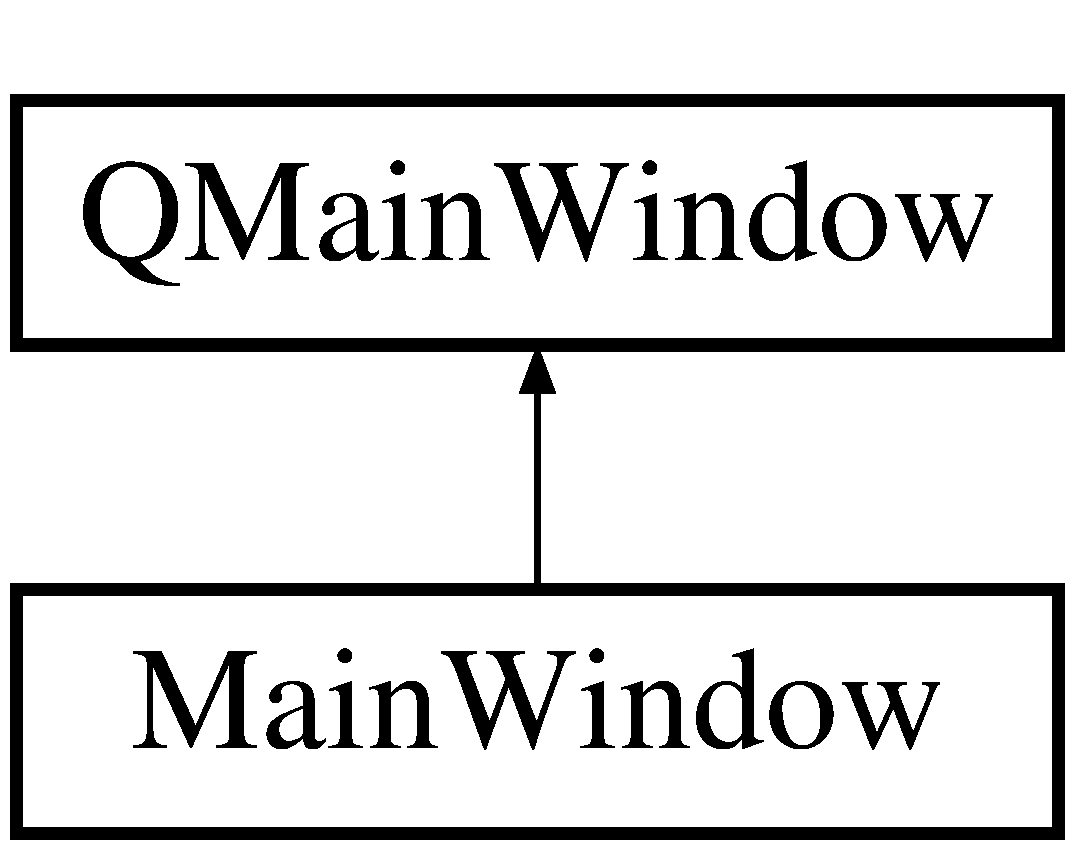
\includegraphics[height=2.000000cm]{class_main_window}
\end{center}
\end{figure}
\subsection*{Public Member Functions}
\begin{DoxyCompactItemize}
\item 
\mbox{\hyperlink{class_main_window_a996c5a2b6f77944776856f08ec30858d}{Main\+Window}} (Q\+Widget $\ast$parent=nullptr)
\item 
\mbox{\hyperlink{class_main_window_ae98d00a93bc118200eeef9f9bba1dba7}{$\sim$\+Main\+Window}} ()
\end{DoxyCompactItemize}
\subsection*{Private Slots}
\begin{DoxyCompactItemize}
\item 
void \mbox{\hyperlink{class_main_window_a680f2fc34bd2147a3a675060aca0fbc6}{on\+Reset\+Button\+Clicked}} ()
\begin{DoxyCompactList}\small\item\em Enters Reset button event. \end{DoxyCompactList}\item 
void \mbox{\hyperlink{class_main_window_ac895c6f8aae08ca6debe77314d640936}{on\+Calibrate\+Button\+Clicked}} ()
\begin{DoxyCompactList}\small\item\em Enters Calibrate button event. \end{DoxyCompactList}\item 
void \mbox{\hyperlink{class_main_window_a92ea4484e5fd9b2d41fe08d2aef4c459}{event\+Loop}} ()
\begin{DoxyCompactList}\small\item\em Repeats events such as\+: reading from serial port, updating rotation and distance values and updating charts. \end{DoxyCompactList}\item 
void \mbox{\hyperlink{class_main_window_aa23e4e2f222120878dc47b594292bb8c}{close\+App\+Event}} ()
\begin{DoxyCompactList}\small\item\em Closes application. \end{DoxyCompactList}\item 
void \mbox{\hyperlink{class_main_window_a3546900c922ca780ef575dd9aa8f9906}{on\+Connect\+Button\+Clicked}} ()
\begin{DoxyCompactList}\small\item\em Connects to the device using serial connection. \end{DoxyCompactList}\item 
void \mbox{\hyperlink{class_main_window_a0a8956278b58c085e0ff06d2edcd739c}{on\+Auto\+Button\+Clicked}} ()
\begin{DoxyCompactList}\small\item\em Automatically looks for proper device. \end{DoxyCompactList}\item 
void \mbox{\hyperlink{class_main_window_a15190e6af528cd13ddbe387800531ba4}{on\+Disconnect\+Button\+Clicked}} ()
\begin{DoxyCompactList}\small\item\em Disconnects from the device. \end{DoxyCompactList}\item 
void \mbox{\hyperlink{class_main_window_ac7fc0a361faba82837af50f2dd1b4ef4}{write\+To\+Status\+Bar}} ()
\begin{DoxyCompactList}\small\item\em Updates status bar text. \end{DoxyCompactList}\end{DoxyCompactItemize}
\subsection*{Private Member Functions}
\begin{DoxyCompactItemize}
\item 
void \mbox{\hyperlink{class_main_window_a9a1bad7a80ca8e1c5075d80143957754}{set\+Graphs\+Properties}} ()
\begin{DoxyCompactList}\small\item\em Sets graphs properties like bg and fg colors and amount of plots. \end{DoxyCompactList}\item 
void \mbox{\hyperlink{class_main_window_aa7a185d6aecfa15957d6fbfa0c42330b}{generate\+Bar\+Graph}} (Q\+Custom\+Plot $\ast$pointer, const Q\+Vector$<$ double $>$ \&data, const quint32 \&\mbox{\hyperlink{class_main_window_a390ce6d302bff7952eee7d92a6cf3da3}{plots\+Amount}}, const Q\+Vector$<$ Q\+String $>$ \&labels, const Q\+Color \&\mbox{\hyperlink{class_main_window_a4a1005daadc7447af6907c57b54e41ab}{bg\+Color}}, const Q\+Color \&\mbox{\hyperlink{class_main_window_a1f5455abfb51d7c4733bfad76ac60606}{fg\+Color}})
\begin{DoxyCompactList}\small\item\em Generates bar graph. \end{DoxyCompactList}\item 
void \mbox{\hyperlink{class_main_window_a1e61f5c68914afa9a1054cbb9982cf17}{update\+Bar\+Graph}} (Q\+Custom\+Plot $\ast$pointer, const Q\+Vector$<$ double $>$ \&data, const quint32 \&\mbox{\hyperlink{class_main_window_a390ce6d302bff7952eee7d92a6cf3da3}{plots\+Amount}}, const Q\+Vector$<$ Q\+String $>$ \&labels, const Q\+Color \&\mbox{\hyperlink{class_main_window_a4a1005daadc7447af6907c57b54e41ab}{bg\+Color}}, const Q\+Color \&\mbox{\hyperlink{class_main_window_a1f5455abfb51d7c4733bfad76ac60606}{fg\+Color}})
\begin{DoxyCompactList}\small\item\em Updated bar graph. \end{DoxyCompactList}\item 
void \mbox{\hyperlink{class_main_window_a2f9acdc998f6f84d2b14d7feda97133c}{generate\+Linear\+Graph}} (Q\+Custom\+Plot $\ast$pointer, const quint32 \&\mbox{\hyperlink{class_main_window_a390ce6d302bff7952eee7d92a6cf3da3}{plots\+Amount}}, const Q\+Vector$<$ Q\+String $>$ \&labels, const Q\+Vector$<$ Q\+String $>$ \&\mbox{\hyperlink{class_main_window_a80e2a1a6949dc004e0729bdb133497dd}{legend}}, const Q\+Vector$<$ Q\+Color $>$ \&\mbox{\hyperlink{class_main_window_af05a0194c683ce9a5abb789e636494da}{plot\+Colors}}, const Q\+Color \&\mbox{\hyperlink{class_main_window_a4a1005daadc7447af6907c57b54e41ab}{bg\+Color}}, const Q\+Color \&\mbox{\hyperlink{class_main_window_a1f5455abfb51d7c4733bfad76ac60606}{fg\+Color}})
\begin{DoxyCompactList}\small\item\em Generates linear graph. \end{DoxyCompactList}\item 
void \mbox{\hyperlink{class_main_window_a26aa34275169fb8830c03b47e97ff0ea}{update\+Linear\+Graph}} (Q\+Custom\+Plot $\ast$pointer, const Q\+Vector$<$ Q\+Vector$<$ double $>$ $\ast$$>$ pointers, const quint32 \&\mbox{\hyperlink{class_main_window_a390ce6d302bff7952eee7d92a6cf3da3}{plots\+Amount}})
\begin{DoxyCompactList}\small\item\em Updated linear graph. \end{DoxyCompactList}\item 
void \mbox{\hyperlink{class_main_window_ab7febfbc2493e928eea3beba33b4b6bb}{clear\+History\+Plots}} ()
\begin{DoxyCompactList}\small\item\em Clears measurements history data. \end{DoxyCompactList}\item 
void \mbox{\hyperlink{class_main_window_ae9a461c9fd369552f0e8871ec8f8f191}{clear\+Realtime\+Plots}} ()
\begin{DoxyCompactList}\small\item\em Clears real time data. \end{DoxyCompactList}\item 
void \mbox{\hyperlink{class_main_window_ad5f5900379db4ae670ad541da8f55384}{set\+Combo\+Box}} ()
\begin{DoxyCompactList}\small\item\em Sets combo box. \end{DoxyCompactList}\item 
Q\+String \mbox{\hyperlink{class_main_window_a5c8dccfe7131cf3c08ff9cbb9ff642d4}{get\+Error\+Text}} (const quint32 error\+Code) const
\begin{DoxyCompactList}\small\item\em Returns specific error\textquotesingle{}s text based on error\textquotesingle{}s code. \end{DoxyCompactList}\item 
void \mbox{\hyperlink{class_main_window_a366da6a45407c523f570ca9e4f4b40a4}{show\+Message}} ()
\begin{DoxyCompactList}\small\item\em Shows message on status bar based on arduino. \end{DoxyCompactList}\item 
void \mbox{\hyperlink{class_main_window_a365152de4a1878ab0087816da6a9431a}{show\+Message}} (const quint32 error\+Code)
\begin{DoxyCompactList}\small\item\em Shows message on status bar based on error\textquotesingle{}s code. \end{DoxyCompactList}\end{DoxyCompactItemize}
\subsection*{Private Attributes}
\begin{DoxyCompactItemize}
\item 
\mbox{\hyperlink{class_measurement_handler}{Measurement\+Handler}} $\ast$ \mbox{\hyperlink{class_main_window_a6a921ce08975d864ff158f36760802a8}{transform}}
\item 
\mbox{\hyperlink{class_serial_port_reader}{Serial\+Port\+Reader}} $\ast$ \mbox{\hyperlink{class_main_window_aba5a40e0587b38a584b92583600373f6}{arduino}}
\item 
Ui\+::\+Main\+Window $\ast$ \mbox{\hyperlink{class_main_window_a35466a70ed47252a0191168126a352a5}{ui}}
\item 
Q\+Timer \mbox{\hyperlink{class_main_window_a623ca812f462c5bc27daf8a94cff59d1}{loop\+Timer}}
\item 
Q\+Timer \mbox{\hyperlink{class_main_window_af66c315b651ade2e54045edb68c51c86}{status\+Bar\+Timer}}
\item 
Q\+Vector$<$ Q\+String $>$ \mbox{\hyperlink{class_main_window_a9243762b319de95b998df3e36934d6ef}{labels1}}
\item 
Q\+Vector$<$ Q\+String $>$ \mbox{\hyperlink{class_main_window_a81d3e91905b239abfc54858b2954b7f7}{labels2}}
\item 
Q\+Vector$<$ Q\+String $>$ \mbox{\hyperlink{class_main_window_ab9b1318826e6722ec4a5dd99cd0ae353}{labels3}}
\item 
Q\+Vector$<$ Q\+String $>$ \mbox{\hyperlink{class_main_window_a513d5d910d4ece239f1a25d6240869ce}{labels4}}
\item 
Q\+Vector$<$ Q\+String $>$ \mbox{\hyperlink{class_main_window_a80e2a1a6949dc004e0729bdb133497dd}{legend}}
\item 
Q\+Vector$<$ Q\+Color $>$ \mbox{\hyperlink{class_main_window_af05a0194c683ce9a5abb789e636494da}{plot\+Colors}}
\item 
Q\+Color \mbox{\hyperlink{class_main_window_a4a1005daadc7447af6907c57b54e41ab}{bg\+Color}}
\item 
Q\+Color \mbox{\hyperlink{class_main_window_a1f5455abfb51d7c4733bfad76ac60606}{fg\+Color}}
\item 
quint32 \mbox{\hyperlink{class_main_window_a390ce6d302bff7952eee7d92a6cf3da3}{plots\+Amount}}
\item 
double \mbox{\hyperlink{class_main_window_a79199e3cec2bb50434f184cc762bce2e}{max\+Y\+Axis\+Value}}
\item 
double \mbox{\hyperlink{class_main_window_a5cbbcacb99514a12d6743ebb45836f12}{max\+Y\+Axis\+Value2}}
\end{DoxyCompactItemize}


\subsection{Detailed Description}
A class that supports the user interface and a module that generates charts. 

\subsection{Constructor \& Destructor Documentation}
\mbox{\Hypertarget{class_main_window_a996c5a2b6f77944776856f08ec30858d}\label{class_main_window_a996c5a2b6f77944776856f08ec30858d}} 
\index{Main\+Window@{Main\+Window}!Main\+Window@{Main\+Window}}
\index{Main\+Window@{Main\+Window}!Main\+Window@{Main\+Window}}
\subsubsection{\texorpdfstring{Main\+Window()}{MainWindow()}}
{\footnotesize\ttfamily Main\+Window\+::\+Main\+Window (\begin{DoxyParamCaption}\item[{Q\+Widget $\ast$}]{parent = {\ttfamily nullptr} }\end{DoxyParamCaption})\hspace{0.3cm}{\ttfamily [explicit]}}

\mbox{\Hypertarget{class_main_window_ae98d00a93bc118200eeef9f9bba1dba7}\label{class_main_window_ae98d00a93bc118200eeef9f9bba1dba7}} 
\index{Main\+Window@{Main\+Window}!````~Main\+Window@{$\sim$\+Main\+Window}}
\index{````~Main\+Window@{$\sim$\+Main\+Window}!Main\+Window@{Main\+Window}}
\subsubsection{\texorpdfstring{$\sim$\+Main\+Window()}{~MainWindow()}}
{\footnotesize\ttfamily Main\+Window\+::$\sim$\+Main\+Window (\begin{DoxyParamCaption}{ }\end{DoxyParamCaption})}



\subsection{Member Function Documentation}
\mbox{\Hypertarget{class_main_window_ab7febfbc2493e928eea3beba33b4b6bb}\label{class_main_window_ab7febfbc2493e928eea3beba33b4b6bb}} 
\index{Main\+Window@{Main\+Window}!clear\+History\+Plots@{clear\+History\+Plots}}
\index{clear\+History\+Plots@{clear\+History\+Plots}!Main\+Window@{Main\+Window}}
\subsubsection{\texorpdfstring{clear\+History\+Plots()}{clearHistoryPlots()}}
{\footnotesize\ttfamily void Main\+Window\+::clear\+History\+Plots (\begin{DoxyParamCaption}{ }\end{DoxyParamCaption})\hspace{0.3cm}{\ttfamily [private]}}



Clears measurements history data. 

\mbox{\Hypertarget{class_main_window_ae9a461c9fd369552f0e8871ec8f8f191}\label{class_main_window_ae9a461c9fd369552f0e8871ec8f8f191}} 
\index{Main\+Window@{Main\+Window}!clear\+Realtime\+Plots@{clear\+Realtime\+Plots}}
\index{clear\+Realtime\+Plots@{clear\+Realtime\+Plots}!Main\+Window@{Main\+Window}}
\subsubsection{\texorpdfstring{clear\+Realtime\+Plots()}{clearRealtimePlots()}}
{\footnotesize\ttfamily void Main\+Window\+::clear\+Realtime\+Plots (\begin{DoxyParamCaption}{ }\end{DoxyParamCaption})\hspace{0.3cm}{\ttfamily [private]}}



Clears real time data. 

\mbox{\Hypertarget{class_main_window_aa23e4e2f222120878dc47b594292bb8c}\label{class_main_window_aa23e4e2f222120878dc47b594292bb8c}} 
\index{Main\+Window@{Main\+Window}!close\+App\+Event@{close\+App\+Event}}
\index{close\+App\+Event@{close\+App\+Event}!Main\+Window@{Main\+Window}}
\subsubsection{\texorpdfstring{close\+App\+Event}{closeAppEvent}}
{\footnotesize\ttfamily void Main\+Window\+::close\+App\+Event (\begin{DoxyParamCaption}{ }\end{DoxyParamCaption})\hspace{0.3cm}{\ttfamily [private]}, {\ttfamily [slot]}}



Closes application. 

\mbox{\Hypertarget{class_main_window_a92ea4484e5fd9b2d41fe08d2aef4c459}\label{class_main_window_a92ea4484e5fd9b2d41fe08d2aef4c459}} 
\index{Main\+Window@{Main\+Window}!event\+Loop@{event\+Loop}}
\index{event\+Loop@{event\+Loop}!Main\+Window@{Main\+Window}}
\subsubsection{\texorpdfstring{event\+Loop}{eventLoop}}
{\footnotesize\ttfamily void Main\+Window\+::event\+Loop (\begin{DoxyParamCaption}{ }\end{DoxyParamCaption})\hspace{0.3cm}{\ttfamily [private]}, {\ttfamily [slot]}}



Repeats events such as\+: reading from serial port, updating rotation and distance values and updating charts. 

\mbox{\Hypertarget{class_main_window_aa7a185d6aecfa15957d6fbfa0c42330b}\label{class_main_window_aa7a185d6aecfa15957d6fbfa0c42330b}} 
\index{Main\+Window@{Main\+Window}!generate\+Bar\+Graph@{generate\+Bar\+Graph}}
\index{generate\+Bar\+Graph@{generate\+Bar\+Graph}!Main\+Window@{Main\+Window}}
\subsubsection{\texorpdfstring{generate\+Bar\+Graph()}{generateBarGraph()}}
{\footnotesize\ttfamily void Main\+Window\+::generate\+Bar\+Graph (\begin{DoxyParamCaption}\item[{Q\+Custom\+Plot $\ast$}]{pointer,  }\item[{const Q\+Vector$<$ double $>$ \&}]{data,  }\item[{const quint32 \&}]{plots\+Amount,  }\item[{const Q\+Vector$<$ Q\+String $>$ \&}]{labels,  }\item[{const Q\+Color \&}]{bg\+Color,  }\item[{const Q\+Color \&}]{fg\+Color }\end{DoxyParamCaption})\hspace{0.3cm}{\ttfamily [private]}}



Generates bar graph. 


\begin{DoxyParams}{Parameters}
{\em pointer} & -\/ pointer to target widget \\
\hline
{\em data} & -\/ data to plot \\
\hline
{\em plots\+Amount} & -\/ plots amount \\
\hline
{\em labels} & -\/ labels for axes \\
\hline
{\em bg\+Color} & -\/ background color \\
\hline
{\em fg\+Color} & -\/ foreground color \\
\hline
\end{DoxyParams}
\mbox{\Hypertarget{class_main_window_a2f9acdc998f6f84d2b14d7feda97133c}\label{class_main_window_a2f9acdc998f6f84d2b14d7feda97133c}} 
\index{Main\+Window@{Main\+Window}!generate\+Linear\+Graph@{generate\+Linear\+Graph}}
\index{generate\+Linear\+Graph@{generate\+Linear\+Graph}!Main\+Window@{Main\+Window}}
\subsubsection{\texorpdfstring{generate\+Linear\+Graph()}{generateLinearGraph()}}
{\footnotesize\ttfamily void Main\+Window\+::generate\+Linear\+Graph (\begin{DoxyParamCaption}\item[{Q\+Custom\+Plot $\ast$}]{pointer,  }\item[{const quint32 \&}]{plots\+Amount,  }\item[{const Q\+Vector$<$ Q\+String $>$ \&}]{labels,  }\item[{const Q\+Vector$<$ Q\+String $>$ \&}]{legend,  }\item[{const Q\+Vector$<$ Q\+Color $>$ \&}]{plot\+Colors,  }\item[{const Q\+Color \&}]{bg\+Color,  }\item[{const Q\+Color \&}]{fg\+Color }\end{DoxyParamCaption})\hspace{0.3cm}{\ttfamily [private]}}



Generates linear graph. 


\begin{DoxyParams}{Parameters}
{\em pointer} & -\/ pointer to target widget \\
\hline
{\em plots\+Amount} & -\/ plots amount \\
\hline
{\em labels} & -\/ labels for axes \\
\hline
{\em legend} & -\/ legend\textquotesingle{}s text \\
\hline
{\em plot\+Colors} & -\/ plot\textquotesingle{}s colors \\
\hline
{\em bg\+Color} & -\/ background color \\
\hline
{\em fg\+Color} & -\/ foreground color \\
\hline
\end{DoxyParams}
\mbox{\Hypertarget{class_main_window_a5c8dccfe7131cf3c08ff9cbb9ff642d4}\label{class_main_window_a5c8dccfe7131cf3c08ff9cbb9ff642d4}} 
\index{Main\+Window@{Main\+Window}!get\+Error\+Text@{get\+Error\+Text}}
\index{get\+Error\+Text@{get\+Error\+Text}!Main\+Window@{Main\+Window}}
\subsubsection{\texorpdfstring{get\+Error\+Text()}{getErrorText()}}
{\footnotesize\ttfamily Q\+String Main\+Window\+::get\+Error\+Text (\begin{DoxyParamCaption}\item[{const quint32}]{error\+Code }\end{DoxyParamCaption}) const\hspace{0.3cm}{\ttfamily [private]}}



Returns specific error\textquotesingle{}s text based on error\textquotesingle{}s code. 


\begin{DoxyParams}{Parameters}
{\em error\+Code} & -\/ error\textquotesingle{}s code \\
\hline
\end{DoxyParams}
\begin{DoxyReturn}{Returns}
Error\textquotesingle{}s text 
\end{DoxyReturn}
\mbox{\Hypertarget{class_main_window_a0a8956278b58c085e0ff06d2edcd739c}\label{class_main_window_a0a8956278b58c085e0ff06d2edcd739c}} 
\index{Main\+Window@{Main\+Window}!on\+Auto\+Button\+Clicked@{on\+Auto\+Button\+Clicked}}
\index{on\+Auto\+Button\+Clicked@{on\+Auto\+Button\+Clicked}!Main\+Window@{Main\+Window}}
\subsubsection{\texorpdfstring{on\+Auto\+Button\+Clicked}{onAutoButtonClicked}}
{\footnotesize\ttfamily void Main\+Window\+::on\+Auto\+Button\+Clicked (\begin{DoxyParamCaption}{ }\end{DoxyParamCaption})\hspace{0.3cm}{\ttfamily [private]}, {\ttfamily [slot]}}



Automatically looks for proper device. 

\mbox{\Hypertarget{class_main_window_ac895c6f8aae08ca6debe77314d640936}\label{class_main_window_ac895c6f8aae08ca6debe77314d640936}} 
\index{Main\+Window@{Main\+Window}!on\+Calibrate\+Button\+Clicked@{on\+Calibrate\+Button\+Clicked}}
\index{on\+Calibrate\+Button\+Clicked@{on\+Calibrate\+Button\+Clicked}!Main\+Window@{Main\+Window}}
\subsubsection{\texorpdfstring{on\+Calibrate\+Button\+Clicked}{onCalibrateButtonClicked}}
{\footnotesize\ttfamily void Main\+Window\+::on\+Calibrate\+Button\+Clicked (\begin{DoxyParamCaption}{ }\end{DoxyParamCaption})\hspace{0.3cm}{\ttfamily [private]}, {\ttfamily [slot]}}



Enters Calibrate button event. 

\mbox{\Hypertarget{class_main_window_a3546900c922ca780ef575dd9aa8f9906}\label{class_main_window_a3546900c922ca780ef575dd9aa8f9906}} 
\index{Main\+Window@{Main\+Window}!on\+Connect\+Button\+Clicked@{on\+Connect\+Button\+Clicked}}
\index{on\+Connect\+Button\+Clicked@{on\+Connect\+Button\+Clicked}!Main\+Window@{Main\+Window}}
\subsubsection{\texorpdfstring{on\+Connect\+Button\+Clicked}{onConnectButtonClicked}}
{\footnotesize\ttfamily void Main\+Window\+::on\+Connect\+Button\+Clicked (\begin{DoxyParamCaption}{ }\end{DoxyParamCaption})\hspace{0.3cm}{\ttfamily [private]}, {\ttfamily [slot]}}



Connects to the device using serial connection. 

\mbox{\Hypertarget{class_main_window_a15190e6af528cd13ddbe387800531ba4}\label{class_main_window_a15190e6af528cd13ddbe387800531ba4}} 
\index{Main\+Window@{Main\+Window}!on\+Disconnect\+Button\+Clicked@{on\+Disconnect\+Button\+Clicked}}
\index{on\+Disconnect\+Button\+Clicked@{on\+Disconnect\+Button\+Clicked}!Main\+Window@{Main\+Window}}
\subsubsection{\texorpdfstring{on\+Disconnect\+Button\+Clicked}{onDisconnectButtonClicked}}
{\footnotesize\ttfamily void Main\+Window\+::on\+Disconnect\+Button\+Clicked (\begin{DoxyParamCaption}{ }\end{DoxyParamCaption})\hspace{0.3cm}{\ttfamily [private]}, {\ttfamily [slot]}}



Disconnects from the device. 

\mbox{\Hypertarget{class_main_window_a680f2fc34bd2147a3a675060aca0fbc6}\label{class_main_window_a680f2fc34bd2147a3a675060aca0fbc6}} 
\index{Main\+Window@{Main\+Window}!on\+Reset\+Button\+Clicked@{on\+Reset\+Button\+Clicked}}
\index{on\+Reset\+Button\+Clicked@{on\+Reset\+Button\+Clicked}!Main\+Window@{Main\+Window}}
\subsubsection{\texorpdfstring{on\+Reset\+Button\+Clicked}{onResetButtonClicked}}
{\footnotesize\ttfamily void Main\+Window\+::on\+Reset\+Button\+Clicked (\begin{DoxyParamCaption}{ }\end{DoxyParamCaption})\hspace{0.3cm}{\ttfamily [private]}, {\ttfamily [slot]}}



Enters Reset button event. 

\mbox{\Hypertarget{class_main_window_ad5f5900379db4ae670ad541da8f55384}\label{class_main_window_ad5f5900379db4ae670ad541da8f55384}} 
\index{Main\+Window@{Main\+Window}!set\+Combo\+Box@{set\+Combo\+Box}}
\index{set\+Combo\+Box@{set\+Combo\+Box}!Main\+Window@{Main\+Window}}
\subsubsection{\texorpdfstring{set\+Combo\+Box()}{setComboBox()}}
{\footnotesize\ttfamily void Main\+Window\+::set\+Combo\+Box (\begin{DoxyParamCaption}{ }\end{DoxyParamCaption})\hspace{0.3cm}{\ttfamily [private]}}



Sets combo box. 

\mbox{\Hypertarget{class_main_window_a9a1bad7a80ca8e1c5075d80143957754}\label{class_main_window_a9a1bad7a80ca8e1c5075d80143957754}} 
\index{Main\+Window@{Main\+Window}!set\+Graphs\+Properties@{set\+Graphs\+Properties}}
\index{set\+Graphs\+Properties@{set\+Graphs\+Properties}!Main\+Window@{Main\+Window}}
\subsubsection{\texorpdfstring{set\+Graphs\+Properties()}{setGraphsProperties()}}
{\footnotesize\ttfamily void Main\+Window\+::set\+Graphs\+Properties (\begin{DoxyParamCaption}{ }\end{DoxyParamCaption})\hspace{0.3cm}{\ttfamily [private]}}



Sets graphs properties like bg and fg colors and amount of plots. 

\mbox{\Hypertarget{class_main_window_a366da6a45407c523f570ca9e4f4b40a4}\label{class_main_window_a366da6a45407c523f570ca9e4f4b40a4}} 
\index{Main\+Window@{Main\+Window}!show\+Message@{show\+Message}}
\index{show\+Message@{show\+Message}!Main\+Window@{Main\+Window}}
\subsubsection{\texorpdfstring{show\+Message()}{showMessage()}\hspace{0.1cm}{\footnotesize\ttfamily [1/2]}}
{\footnotesize\ttfamily void Main\+Window\+::show\+Message (\begin{DoxyParamCaption}{ }\end{DoxyParamCaption})\hspace{0.3cm}{\ttfamily [private]}}



Shows message on status bar based on arduino. 

\mbox{\Hypertarget{class_main_window_a365152de4a1878ab0087816da6a9431a}\label{class_main_window_a365152de4a1878ab0087816da6a9431a}} 
\index{Main\+Window@{Main\+Window}!show\+Message@{show\+Message}}
\index{show\+Message@{show\+Message}!Main\+Window@{Main\+Window}}
\subsubsection{\texorpdfstring{show\+Message()}{showMessage()}\hspace{0.1cm}{\footnotesize\ttfamily [2/2]}}
{\footnotesize\ttfamily void Main\+Window\+::show\+Message (\begin{DoxyParamCaption}\item[{const quint32}]{error\+Code }\end{DoxyParamCaption})\hspace{0.3cm}{\ttfamily [private]}}



Shows message on status bar based on error\textquotesingle{}s code. 


\begin{DoxyParams}{Parameters}
{\em error\+Code} & -\/ error\textquotesingle{}s code \\
\hline
\end{DoxyParams}
\mbox{\Hypertarget{class_main_window_a1e61f5c68914afa9a1054cbb9982cf17}\label{class_main_window_a1e61f5c68914afa9a1054cbb9982cf17}} 
\index{Main\+Window@{Main\+Window}!update\+Bar\+Graph@{update\+Bar\+Graph}}
\index{update\+Bar\+Graph@{update\+Bar\+Graph}!Main\+Window@{Main\+Window}}
\subsubsection{\texorpdfstring{update\+Bar\+Graph()}{updateBarGraph()}}
{\footnotesize\ttfamily void Main\+Window\+::update\+Bar\+Graph (\begin{DoxyParamCaption}\item[{Q\+Custom\+Plot $\ast$}]{pointer,  }\item[{const Q\+Vector$<$ double $>$ \&}]{data,  }\item[{const quint32 \&}]{plots\+Amount,  }\item[{const Q\+Vector$<$ Q\+String $>$ \&}]{labels,  }\item[{const Q\+Color \&}]{bg\+Color,  }\item[{const Q\+Color \&}]{fg\+Color }\end{DoxyParamCaption})\hspace{0.3cm}{\ttfamily [private]}}



Updated bar graph. 


\begin{DoxyParams}{Parameters}
{\em pointer} & -\/ pointer to target widget \\
\hline
{\em data} & -\/ data to plot \\
\hline
{\em plots\+Amount} & -\/ plots amount \\
\hline
{\em labels} & -\/ labels for axes \\
\hline
{\em bg\+Color} & -\/ background color \\
\hline
{\em fg\+Color} & -\/ foreground color \\
\hline
\end{DoxyParams}
\mbox{\Hypertarget{class_main_window_a26aa34275169fb8830c03b47e97ff0ea}\label{class_main_window_a26aa34275169fb8830c03b47e97ff0ea}} 
\index{Main\+Window@{Main\+Window}!update\+Linear\+Graph@{update\+Linear\+Graph}}
\index{update\+Linear\+Graph@{update\+Linear\+Graph}!Main\+Window@{Main\+Window}}
\subsubsection{\texorpdfstring{update\+Linear\+Graph()}{updateLinearGraph()}}
{\footnotesize\ttfamily void Main\+Window\+::update\+Linear\+Graph (\begin{DoxyParamCaption}\item[{Q\+Custom\+Plot $\ast$}]{pointer,  }\item[{const Q\+Vector$<$ Q\+Vector$<$ double $>$ $\ast$$>$}]{pointers,  }\item[{const quint32 \&}]{plots\+Amount }\end{DoxyParamCaption})\hspace{0.3cm}{\ttfamily [private]}}



Updated linear graph. 


\begin{DoxyParams}{Parameters}
{\em pointer} & -\/ pointer to target widget \\
\hline
{\em pointers} & -\/ pointers to time and data containers \\
\hline
{\em plots\+Amount} & -\/ plots amount \\
\hline
\end{DoxyParams}
\mbox{\Hypertarget{class_main_window_ac7fc0a361faba82837af50f2dd1b4ef4}\label{class_main_window_ac7fc0a361faba82837af50f2dd1b4ef4}} 
\index{Main\+Window@{Main\+Window}!write\+To\+Status\+Bar@{write\+To\+Status\+Bar}}
\index{write\+To\+Status\+Bar@{write\+To\+Status\+Bar}!Main\+Window@{Main\+Window}}
\subsubsection{\texorpdfstring{write\+To\+Status\+Bar}{writeToStatusBar}}
{\footnotesize\ttfamily void Main\+Window\+::write\+To\+Status\+Bar (\begin{DoxyParamCaption}{ }\end{DoxyParamCaption})\hspace{0.3cm}{\ttfamily [private]}, {\ttfamily [slot]}}



Updates status bar text. 



\subsection{Member Data Documentation}
\mbox{\Hypertarget{class_main_window_aba5a40e0587b38a584b92583600373f6}\label{class_main_window_aba5a40e0587b38a584b92583600373f6}} 
\index{Main\+Window@{Main\+Window}!arduino@{arduino}}
\index{arduino@{arduino}!Main\+Window@{Main\+Window}}
\subsubsection{\texorpdfstring{arduino}{arduino}}
{\footnotesize\ttfamily \mbox{\hyperlink{class_serial_port_reader}{Serial\+Port\+Reader}}$\ast$ Main\+Window\+::arduino\hspace{0.3cm}{\ttfamily [private]}}

\mbox{\Hypertarget{class_main_window_a4a1005daadc7447af6907c57b54e41ab}\label{class_main_window_a4a1005daadc7447af6907c57b54e41ab}} 
\index{Main\+Window@{Main\+Window}!bg\+Color@{bg\+Color}}
\index{bg\+Color@{bg\+Color}!Main\+Window@{Main\+Window}}
\subsubsection{\texorpdfstring{bg\+Color}{bgColor}}
{\footnotesize\ttfamily Q\+Color Main\+Window\+::bg\+Color\hspace{0.3cm}{\ttfamily [private]}}

\mbox{\Hypertarget{class_main_window_a1f5455abfb51d7c4733bfad76ac60606}\label{class_main_window_a1f5455abfb51d7c4733bfad76ac60606}} 
\index{Main\+Window@{Main\+Window}!fg\+Color@{fg\+Color}}
\index{fg\+Color@{fg\+Color}!Main\+Window@{Main\+Window}}
\subsubsection{\texorpdfstring{fg\+Color}{fgColor}}
{\footnotesize\ttfamily Q\+Color Main\+Window\+::fg\+Color\hspace{0.3cm}{\ttfamily [private]}}

\mbox{\Hypertarget{class_main_window_a9243762b319de95b998df3e36934d6ef}\label{class_main_window_a9243762b319de95b998df3e36934d6ef}} 
\index{Main\+Window@{Main\+Window}!labels1@{labels1}}
\index{labels1@{labels1}!Main\+Window@{Main\+Window}}
\subsubsection{\texorpdfstring{labels1}{labels1}}
{\footnotesize\ttfamily Q\+Vector$<$Q\+String$>$ Main\+Window\+::labels1\hspace{0.3cm}{\ttfamily [private]}}

acceleration chart labels \mbox{\Hypertarget{class_main_window_a81d3e91905b239abfc54858b2954b7f7}\label{class_main_window_a81d3e91905b239abfc54858b2954b7f7}} 
\index{Main\+Window@{Main\+Window}!labels2@{labels2}}
\index{labels2@{labels2}!Main\+Window@{Main\+Window}}
\subsubsection{\texorpdfstring{labels2}{labels2}}
{\footnotesize\ttfamily Q\+Vector$<$Q\+String$>$ Main\+Window\+::labels2\hspace{0.3cm}{\ttfamily [private]}}

angular velcity chart labels \mbox{\Hypertarget{class_main_window_ab9b1318826e6722ec4a5dd99cd0ae353}\label{class_main_window_ab9b1318826e6722ec4a5dd99cd0ae353}} 
\index{Main\+Window@{Main\+Window}!labels3@{labels3}}
\index{labels3@{labels3}!Main\+Window@{Main\+Window}}
\subsubsection{\texorpdfstring{labels3}{labels3}}
{\footnotesize\ttfamily Q\+Vector$<$Q\+String$>$ Main\+Window\+::labels3\hspace{0.3cm}{\ttfamily [private]}}

angle chart labels \mbox{\Hypertarget{class_main_window_a513d5d910d4ece239f1a25d6240869ce}\label{class_main_window_a513d5d910d4ece239f1a25d6240869ce}} 
\index{Main\+Window@{Main\+Window}!labels4@{labels4}}
\index{labels4@{labels4}!Main\+Window@{Main\+Window}}
\subsubsection{\texorpdfstring{labels4}{labels4}}
{\footnotesize\ttfamily Q\+Vector$<$Q\+String$>$ Main\+Window\+::labels4\hspace{0.3cm}{\ttfamily [private]}}

distance chart labels \mbox{\Hypertarget{class_main_window_a80e2a1a6949dc004e0729bdb133497dd}\label{class_main_window_a80e2a1a6949dc004e0729bdb133497dd}} 
\index{Main\+Window@{Main\+Window}!legend@{legend}}
\index{legend@{legend}!Main\+Window@{Main\+Window}}
\subsubsection{\texorpdfstring{legend}{legend}}
{\footnotesize\ttfamily Q\+Vector$<$Q\+String$>$ Main\+Window\+::legend\hspace{0.3cm}{\ttfamily [private]}}

legend\textquotesingle{}s text for linear graphs \mbox{\Hypertarget{class_main_window_a623ca812f462c5bc27daf8a94cff59d1}\label{class_main_window_a623ca812f462c5bc27daf8a94cff59d1}} 
\index{Main\+Window@{Main\+Window}!loop\+Timer@{loop\+Timer}}
\index{loop\+Timer@{loop\+Timer}!Main\+Window@{Main\+Window}}
\subsubsection{\texorpdfstring{loop\+Timer}{loopTimer}}
{\footnotesize\ttfamily Q\+Timer Main\+Window\+::loop\+Timer\hspace{0.3cm}{\ttfamily [private]}}

timer that sets plots refresh frequency \mbox{\Hypertarget{class_main_window_a79199e3cec2bb50434f184cc762bce2e}\label{class_main_window_a79199e3cec2bb50434f184cc762bce2e}} 
\index{Main\+Window@{Main\+Window}!max\+Y\+Axis\+Value@{max\+Y\+Axis\+Value}}
\index{max\+Y\+Axis\+Value@{max\+Y\+Axis\+Value}!Main\+Window@{Main\+Window}}
\subsubsection{\texorpdfstring{max\+Y\+Axis\+Value}{maxYAxisValue}}
{\footnotesize\ttfamily double Main\+Window\+::max\+Y\+Axis\+Value\hspace{0.3cm}{\ttfamily [private]}}

minimal bar graph value showed on vertical axis for angle graph \mbox{\Hypertarget{class_main_window_a5cbbcacb99514a12d6743ebb45836f12}\label{class_main_window_a5cbbcacb99514a12d6743ebb45836f12}} 
\index{Main\+Window@{Main\+Window}!max\+Y\+Axis\+Value2@{max\+Y\+Axis\+Value2}}
\index{max\+Y\+Axis\+Value2@{max\+Y\+Axis\+Value2}!Main\+Window@{Main\+Window}}
\subsubsection{\texorpdfstring{max\+Y\+Axis\+Value2}{maxYAxisValue2}}
{\footnotesize\ttfamily double Main\+Window\+::max\+Y\+Axis\+Value2\hspace{0.3cm}{\ttfamily [private]}}

minimal bar graph value showed on vertical axis for distance graph \mbox{\Hypertarget{class_main_window_af05a0194c683ce9a5abb789e636494da}\label{class_main_window_af05a0194c683ce9a5abb789e636494da}} 
\index{Main\+Window@{Main\+Window}!plot\+Colors@{plot\+Colors}}
\index{plot\+Colors@{plot\+Colors}!Main\+Window@{Main\+Window}}
\subsubsection{\texorpdfstring{plot\+Colors}{plotColors}}
{\footnotesize\ttfamily Q\+Vector$<$Q\+Color$>$ Main\+Window\+::plot\+Colors\hspace{0.3cm}{\ttfamily [private]}}

plot\textquotesingle{}s color for linear graphs \mbox{\Hypertarget{class_main_window_a390ce6d302bff7952eee7d92a6cf3da3}\label{class_main_window_a390ce6d302bff7952eee7d92a6cf3da3}} 
\index{Main\+Window@{Main\+Window}!plots\+Amount@{plots\+Amount}}
\index{plots\+Amount@{plots\+Amount}!Main\+Window@{Main\+Window}}
\subsubsection{\texorpdfstring{plots\+Amount}{plotsAmount}}
{\footnotesize\ttfamily quint32 Main\+Window\+::plots\+Amount\hspace{0.3cm}{\ttfamily [private]}}

\mbox{\Hypertarget{class_main_window_af66c315b651ade2e54045edb68c51c86}\label{class_main_window_af66c315b651ade2e54045edb68c51c86}} 
\index{Main\+Window@{Main\+Window}!status\+Bar\+Timer@{status\+Bar\+Timer}}
\index{status\+Bar\+Timer@{status\+Bar\+Timer}!Main\+Window@{Main\+Window}}
\subsubsection{\texorpdfstring{status\+Bar\+Timer}{statusBarTimer}}
{\footnotesize\ttfamily Q\+Timer Main\+Window\+::status\+Bar\+Timer\hspace{0.3cm}{\ttfamily [private]}}

timer that sets how long will be status bar communicates displayed \mbox{\Hypertarget{class_main_window_a6a921ce08975d864ff158f36760802a8}\label{class_main_window_a6a921ce08975d864ff158f36760802a8}} 
\index{Main\+Window@{Main\+Window}!transform@{transform}}
\index{transform@{transform}!Main\+Window@{Main\+Window}}
\subsubsection{\texorpdfstring{transform}{transform}}
{\footnotesize\ttfamily \mbox{\hyperlink{class_measurement_handler}{Measurement\+Handler}}$\ast$ Main\+Window\+::transform\hspace{0.3cm}{\ttfamily [private]}}

\mbox{\Hypertarget{class_main_window_a35466a70ed47252a0191168126a352a5}\label{class_main_window_a35466a70ed47252a0191168126a352a5}} 
\index{Main\+Window@{Main\+Window}!ui@{ui}}
\index{ui@{ui}!Main\+Window@{Main\+Window}}
\subsubsection{\texorpdfstring{ui}{ui}}
{\footnotesize\ttfamily Ui\+::\+Main\+Window$\ast$ Main\+Window\+::ui\hspace{0.3cm}{\ttfamily [private]}}



The documentation for this class was generated from the following files\+:\begin{DoxyCompactItemize}
\item 
h/\mbox{\hyperlink{mainwindow_8h}{mainwindow.\+h}}\item 
cpp/\mbox{\hyperlink{mainwindow_8cpp}{mainwindow.\+cpp}}\end{DoxyCompactItemize}

\section{Measurement\+Handler Class Reference}
\label{class_measurement_handler}\index{Measurement\+Handler@{Measurement\+Handler}}


A class for storing data from sensors received from the microcontroller and handling necessary conversions.  




{\ttfamily \#include $<$measurementhandler.\+h$>$}

\subsection*{Public Member Functions}
\begin{DoxyCompactItemize}
\item 
\textbf{ Measurement\+Handler} ()
\item 
\textbf{ $\sim$\+Measurement\+Handler} ()
\item 
Q\+Vector$<$ double $>$ $\ast$ \textbf{ get\+Time} () const
\item 
Q\+Vector$<$ double $>$ $\ast$ \textbf{ get\+X\+Acc} () const
\item 
Q\+Vector$<$ double $>$ $\ast$ \textbf{ get\+Y\+Acc} () const
\item 
Q\+Vector$<$ double $>$ $\ast$ \textbf{ get\+Z\+Acc} () const
\item 
Q\+Vector$<$ double $>$ $\ast$ \textbf{ get\+X\+Ang\+Vel} () const
\item 
Q\+Vector$<$ double $>$ $\ast$ \textbf{ get\+Y\+Ang\+Vel} () const
\item 
Q\+Vector$<$ double $>$ $\ast$ \textbf{ get\+Z\+Ang\+Vel} () const
\item 
void \textbf{ push\+Time} (double value)
\item 
void \textbf{ push\+X\+Acc} (double value)
\item 
void \textbf{ push\+Y\+Acc} (double value)
\item 
void \textbf{ push\+Z\+Acc} (double value)
\item 
void \textbf{ push\+X\+Ang\+Vel} (double value)
\item 
void \textbf{ push\+Y\+Ang\+Vel} (double value)
\item 
void \textbf{ push\+Z\+Ang\+Vel} (double value)
\item 
void \textbf{ calc\+Angle\+And\+Distance} ()
\begin{DoxyCompactList}\small\item\em Calculates angle [deg] and distance [cm]. \end{DoxyCompactList}\item 
void \textbf{ clear\+History\+Data} ()
\begin{DoxyCompactList}\small\item\em Deletes angular velocity and linear acceleration data. \end{DoxyCompactList}\item 
void \textbf{ clear\+Realtime\+Data} ()
\begin{DoxyCompactList}\small\item\em Deletes rotation and distance data. \end{DoxyCompactList}\item 
Q\+Vector$<$ double $>$ \textbf{ get\+Acc\+Meas} () const
\item 
Q\+Vector$<$ double $>$ \& \textbf{ set\+Acc\+Meas} ()
\item 
Q\+Vector$<$ double $>$ \textbf{ get\+Gyro\+Meas} () const
\item 
Q\+Vector$<$ double $>$ \& \textbf{ set\+Gyro\+Meas} ()
\item 
Q\+Vector$<$ double $>$ \textbf{ get\+Angle} () const
\item 
Q\+Vector$<$ double $>$ \& \textbf{ set\+Angle} ()
\item 
Q\+Vector$<$ double $>$ \textbf{ get\+Distance} () const
\item 
Q\+Vector$<$ double $>$ \& \textbf{ set\+Distance} ()
\item 
Q\+Vector$<$ Q\+Vector$<$ double $>$ $\ast$ $>$ \textbf{ get\+Vector\+Of\+Acc\+Pointers} () const
\item 
Q\+Vector$<$ Q\+Vector$<$ double $>$ $\ast$ $>$ \textbf{ get\+Vector\+Of\+Gyro\+Pointers} () const
\end{DoxyCompactItemize}
\subsection*{Private Attributes}
\begin{DoxyCompactItemize}
\item 
Q\+Vector$<$ double $>$ $\ast$ \textbf{ time}
\item 
Q\+Vector$<$ double $>$ $\ast$ \textbf{ x\+Acc}
\item 
Q\+Vector$<$ double $>$ $\ast$ \textbf{ y\+Acc}
\item 
Q\+Vector$<$ double $>$ $\ast$ \textbf{ z\+Acc}
\item 
Q\+Vector$<$ double $>$ $\ast$ \textbf{ x\+Ang\+Vel}
\item 
Q\+Vector$<$ double $>$ $\ast$ \textbf{ y\+Ang\+Vel}
\item 
Q\+Vector$<$ double $>$ $\ast$ \textbf{ z\+Ang\+Vel}
\item 
Q\+Vector$<$ double $>$ \textbf{ acc\+Meas}
\item 
Q\+Vector$<$ double $>$ \textbf{ gyro\+Meas}
\item 
Q\+Vector$<$ double $>$ \textbf{ angle}
\item 
Q\+Vector$<$ double $>$ \textbf{ distance}
\item 
Q\+Vector$<$ double $>$ \textbf{ angleP}
\item 
Q\+Vector$<$ double $>$ \textbf{ distanceP}
\item 
Q\+Vector$<$ Q\+Vector$<$ double $>$ $\ast$ $>$ \textbf{ vector\+Of\+Acc\+Pointers}
\item 
Q\+Vector$<$ Q\+Vector$<$ double $>$ $\ast$ $>$ \textbf{ vector\+Of\+Gyro\+Pointers}
\end{DoxyCompactItemize}


\subsection{Detailed Description}
A class for storing data from sensors received from the microcontroller and handling necessary conversions. 

\subsection{Constructor \& Destructor Documentation}
\mbox{\label{class_measurement_handler_a80f0638e83958605b26eb39e4e8a49e4}} 
\index{Measurement\+Handler@{Measurement\+Handler}!Measurement\+Handler@{Measurement\+Handler}}
\index{Measurement\+Handler@{Measurement\+Handler}!Measurement\+Handler@{Measurement\+Handler}}
\subsubsection{Measurement\+Handler()}
{\footnotesize\ttfamily Measurement\+Handler\+::\+Measurement\+Handler (\begin{DoxyParamCaption}{ }\end{DoxyParamCaption})}

\mbox{\label{class_measurement_handler_ab1f1ce3908fc0d88e350727efbd2949a}} 
\index{Measurement\+Handler@{Measurement\+Handler}!````~Measurement\+Handler@{$\sim$\+Measurement\+Handler}}
\index{````~Measurement\+Handler@{$\sim$\+Measurement\+Handler}!Measurement\+Handler@{Measurement\+Handler}}
\subsubsection{$\sim$\+Measurement\+Handler()}
{\footnotesize\ttfamily Measurement\+Handler\+::$\sim$\+Measurement\+Handler (\begin{DoxyParamCaption}{ }\end{DoxyParamCaption})}



\subsection{Member Function Documentation}
\mbox{\label{class_measurement_handler_a1a88ac326f78ba4ee92f4ac16cf3d2dd}} 
\index{Measurement\+Handler@{Measurement\+Handler}!calc\+Angle\+And\+Distance@{calc\+Angle\+And\+Distance}}
\index{calc\+Angle\+And\+Distance@{calc\+Angle\+And\+Distance}!Measurement\+Handler@{Measurement\+Handler}}
\subsubsection{calc\+Angle\+And\+Distance()}
{\footnotesize\ttfamily void Measurement\+Handler\+::calc\+Angle\+And\+Distance (\begin{DoxyParamCaption}{ }\end{DoxyParamCaption})}



Calculates angle [deg] and distance [cm]. 

\mbox{\label{class_measurement_handler_a4287d2123c6307d6d91790efe03f57a2}} 
\index{Measurement\+Handler@{Measurement\+Handler}!clear\+History\+Data@{clear\+History\+Data}}
\index{clear\+History\+Data@{clear\+History\+Data}!Measurement\+Handler@{Measurement\+Handler}}
\subsubsection{clear\+History\+Data()}
{\footnotesize\ttfamily void Measurement\+Handler\+::clear\+History\+Data (\begin{DoxyParamCaption}{ }\end{DoxyParamCaption})}



Deletes angular velocity and linear acceleration data. 

\mbox{\label{class_measurement_handler_a97180ca03e2cbf6735eae197493cb7e9}} 
\index{Measurement\+Handler@{Measurement\+Handler}!clear\+Realtime\+Data@{clear\+Realtime\+Data}}
\index{clear\+Realtime\+Data@{clear\+Realtime\+Data}!Measurement\+Handler@{Measurement\+Handler}}
\subsubsection{clear\+Realtime\+Data()}
{\footnotesize\ttfamily void Measurement\+Handler\+::clear\+Realtime\+Data (\begin{DoxyParamCaption}{ }\end{DoxyParamCaption})}



Deletes rotation and distance data. 

\mbox{\label{class_measurement_handler_a16cda730675bd1c0523327c6fd6a1669}} 
\index{Measurement\+Handler@{Measurement\+Handler}!get\+Acc\+Meas@{get\+Acc\+Meas}}
\index{get\+Acc\+Meas@{get\+Acc\+Meas}!Measurement\+Handler@{Measurement\+Handler}}
\subsubsection{get\+Acc\+Meas()}
{\footnotesize\ttfamily Q\+Vector$<$ double $>$ Measurement\+Handler\+::get\+Acc\+Meas (\begin{DoxyParamCaption}{ }\end{DoxyParamCaption}) const}

\mbox{\label{class_measurement_handler_a95251b5abed0a716be546e4c58f48910}} 
\index{Measurement\+Handler@{Measurement\+Handler}!get\+Angle@{get\+Angle}}
\index{get\+Angle@{get\+Angle}!Measurement\+Handler@{Measurement\+Handler}}
\subsubsection{get\+Angle()}
{\footnotesize\ttfamily Q\+Vector$<$ double $>$ Measurement\+Handler\+::get\+Angle (\begin{DoxyParamCaption}{ }\end{DoxyParamCaption}) const}

\mbox{\label{class_measurement_handler_a4d4422673f5deb300499051df34dec30}} 
\index{Measurement\+Handler@{Measurement\+Handler}!get\+Distance@{get\+Distance}}
\index{get\+Distance@{get\+Distance}!Measurement\+Handler@{Measurement\+Handler}}
\subsubsection{get\+Distance()}
{\footnotesize\ttfamily Q\+Vector$<$ double $>$ Measurement\+Handler\+::get\+Distance (\begin{DoxyParamCaption}{ }\end{DoxyParamCaption}) const}

\mbox{\label{class_measurement_handler_a80a29ba6bdd4aff53041f4c7f6ae90bd}} 
\index{Measurement\+Handler@{Measurement\+Handler}!get\+Gyro\+Meas@{get\+Gyro\+Meas}}
\index{get\+Gyro\+Meas@{get\+Gyro\+Meas}!Measurement\+Handler@{Measurement\+Handler}}
\subsubsection{get\+Gyro\+Meas()}
{\footnotesize\ttfamily Q\+Vector$<$ double $>$ Measurement\+Handler\+::get\+Gyro\+Meas (\begin{DoxyParamCaption}{ }\end{DoxyParamCaption}) const}

\mbox{\label{class_measurement_handler_a202be23096eca6bd4362a9aa5552b4f1}} 
\index{Measurement\+Handler@{Measurement\+Handler}!get\+Time@{get\+Time}}
\index{get\+Time@{get\+Time}!Measurement\+Handler@{Measurement\+Handler}}
\subsubsection{get\+Time()}
{\footnotesize\ttfamily Q\+Vector$<$ double $>$ $\ast$ Measurement\+Handler\+::get\+Time (\begin{DoxyParamCaption}{ }\end{DoxyParamCaption}) const}

\mbox{\label{class_measurement_handler_a18ae7fd0f8f2ed3e74e9a7cb87af92e3}} 
\index{Measurement\+Handler@{Measurement\+Handler}!get\+Vector\+Of\+Acc\+Pointers@{get\+Vector\+Of\+Acc\+Pointers}}
\index{get\+Vector\+Of\+Acc\+Pointers@{get\+Vector\+Of\+Acc\+Pointers}!Measurement\+Handler@{Measurement\+Handler}}
\subsubsection{get\+Vector\+Of\+Acc\+Pointers()}
{\footnotesize\ttfamily Q\+Vector$<$ Q\+Vector$<$ double $>$ $\ast$ $>$ Measurement\+Handler\+::get\+Vector\+Of\+Acc\+Pointers (\begin{DoxyParamCaption}{ }\end{DoxyParamCaption}) const}

\mbox{\label{class_measurement_handler_a15b2c74a4325c0ade1dd92f2b4afdabd}} 
\index{Measurement\+Handler@{Measurement\+Handler}!get\+Vector\+Of\+Gyro\+Pointers@{get\+Vector\+Of\+Gyro\+Pointers}}
\index{get\+Vector\+Of\+Gyro\+Pointers@{get\+Vector\+Of\+Gyro\+Pointers}!Measurement\+Handler@{Measurement\+Handler}}
\subsubsection{get\+Vector\+Of\+Gyro\+Pointers()}
{\footnotesize\ttfamily Q\+Vector$<$ Q\+Vector$<$ double $>$ $\ast$ $>$ Measurement\+Handler\+::get\+Vector\+Of\+Gyro\+Pointers (\begin{DoxyParamCaption}{ }\end{DoxyParamCaption}) const}

\mbox{\label{class_measurement_handler_a4dd297cf8cc08203264492496b4378ee}} 
\index{Measurement\+Handler@{Measurement\+Handler}!get\+X\+Acc@{get\+X\+Acc}}
\index{get\+X\+Acc@{get\+X\+Acc}!Measurement\+Handler@{Measurement\+Handler}}
\subsubsection{get\+X\+Acc()}
{\footnotesize\ttfamily Q\+Vector$<$ double $>$ $\ast$ Measurement\+Handler\+::get\+X\+Acc (\begin{DoxyParamCaption}{ }\end{DoxyParamCaption}) const}

\mbox{\label{class_measurement_handler_ae5930434d2c8d66ac124f996fa9fd12d}} 
\index{Measurement\+Handler@{Measurement\+Handler}!get\+X\+Ang\+Vel@{get\+X\+Ang\+Vel}}
\index{get\+X\+Ang\+Vel@{get\+X\+Ang\+Vel}!Measurement\+Handler@{Measurement\+Handler}}
\subsubsection{get\+X\+Ang\+Vel()}
{\footnotesize\ttfamily Q\+Vector$<$ double $>$ $\ast$ Measurement\+Handler\+::get\+X\+Ang\+Vel (\begin{DoxyParamCaption}{ }\end{DoxyParamCaption}) const}

\mbox{\label{class_measurement_handler_a1c7cc1cd1c7e6a1629ad62877e22bd00}} 
\index{Measurement\+Handler@{Measurement\+Handler}!get\+Y\+Acc@{get\+Y\+Acc}}
\index{get\+Y\+Acc@{get\+Y\+Acc}!Measurement\+Handler@{Measurement\+Handler}}
\subsubsection{get\+Y\+Acc()}
{\footnotesize\ttfamily Q\+Vector$<$ double $>$ $\ast$ Measurement\+Handler\+::get\+Y\+Acc (\begin{DoxyParamCaption}{ }\end{DoxyParamCaption}) const}

\mbox{\label{class_measurement_handler_ae2053ba8ad1924ff0ad7c2538da7a35e}} 
\index{Measurement\+Handler@{Measurement\+Handler}!get\+Y\+Ang\+Vel@{get\+Y\+Ang\+Vel}}
\index{get\+Y\+Ang\+Vel@{get\+Y\+Ang\+Vel}!Measurement\+Handler@{Measurement\+Handler}}
\subsubsection{get\+Y\+Ang\+Vel()}
{\footnotesize\ttfamily Q\+Vector$<$ double $>$ $\ast$ Measurement\+Handler\+::get\+Y\+Ang\+Vel (\begin{DoxyParamCaption}{ }\end{DoxyParamCaption}) const}

\mbox{\label{class_measurement_handler_aa9429cbbd110d64168635e9325dcf487}} 
\index{Measurement\+Handler@{Measurement\+Handler}!get\+Z\+Acc@{get\+Z\+Acc}}
\index{get\+Z\+Acc@{get\+Z\+Acc}!Measurement\+Handler@{Measurement\+Handler}}
\subsubsection{get\+Z\+Acc()}
{\footnotesize\ttfamily Q\+Vector$<$ double $>$ $\ast$ Measurement\+Handler\+::get\+Z\+Acc (\begin{DoxyParamCaption}{ }\end{DoxyParamCaption}) const}

\mbox{\label{class_measurement_handler_a89631c6b8b3ba7c1aab620bdcf595896}} 
\index{Measurement\+Handler@{Measurement\+Handler}!get\+Z\+Ang\+Vel@{get\+Z\+Ang\+Vel}}
\index{get\+Z\+Ang\+Vel@{get\+Z\+Ang\+Vel}!Measurement\+Handler@{Measurement\+Handler}}
\subsubsection{get\+Z\+Ang\+Vel()}
{\footnotesize\ttfamily Q\+Vector$<$ double $>$ $\ast$ Measurement\+Handler\+::get\+Z\+Ang\+Vel (\begin{DoxyParamCaption}{ }\end{DoxyParamCaption}) const}

\mbox{\label{class_measurement_handler_a95dad9123275dbb03f9cd01852e82df5}} 
\index{Measurement\+Handler@{Measurement\+Handler}!push\+Time@{push\+Time}}
\index{push\+Time@{push\+Time}!Measurement\+Handler@{Measurement\+Handler}}
\subsubsection{push\+Time()}
{\footnotesize\ttfamily void Measurement\+Handler\+::push\+Time (\begin{DoxyParamCaption}\item[{double}]{value }\end{DoxyParamCaption})}

\mbox{\label{class_measurement_handler_a73435da23551d54e3db30467a0d7d82a}} 
\index{Measurement\+Handler@{Measurement\+Handler}!push\+X\+Acc@{push\+X\+Acc}}
\index{push\+X\+Acc@{push\+X\+Acc}!Measurement\+Handler@{Measurement\+Handler}}
\subsubsection{push\+X\+Acc()}
{\footnotesize\ttfamily void Measurement\+Handler\+::push\+X\+Acc (\begin{DoxyParamCaption}\item[{double}]{value }\end{DoxyParamCaption})}

\mbox{\label{class_measurement_handler_ad0cd4fa68261258a586ae193be1055ba}} 
\index{Measurement\+Handler@{Measurement\+Handler}!push\+X\+Ang\+Vel@{push\+X\+Ang\+Vel}}
\index{push\+X\+Ang\+Vel@{push\+X\+Ang\+Vel}!Measurement\+Handler@{Measurement\+Handler}}
\subsubsection{push\+X\+Ang\+Vel()}
{\footnotesize\ttfamily void Measurement\+Handler\+::push\+X\+Ang\+Vel (\begin{DoxyParamCaption}\item[{double}]{value }\end{DoxyParamCaption})}

\mbox{\label{class_measurement_handler_a43008204cdec1e632d2da7d76b6351af}} 
\index{Measurement\+Handler@{Measurement\+Handler}!push\+Y\+Acc@{push\+Y\+Acc}}
\index{push\+Y\+Acc@{push\+Y\+Acc}!Measurement\+Handler@{Measurement\+Handler}}
\subsubsection{push\+Y\+Acc()}
{\footnotesize\ttfamily void Measurement\+Handler\+::push\+Y\+Acc (\begin{DoxyParamCaption}\item[{double}]{value }\end{DoxyParamCaption})}

\mbox{\label{class_measurement_handler_a51a85f65ef2ca40ad069d66d3a770a57}} 
\index{Measurement\+Handler@{Measurement\+Handler}!push\+Y\+Ang\+Vel@{push\+Y\+Ang\+Vel}}
\index{push\+Y\+Ang\+Vel@{push\+Y\+Ang\+Vel}!Measurement\+Handler@{Measurement\+Handler}}
\subsubsection{push\+Y\+Ang\+Vel()}
{\footnotesize\ttfamily void Measurement\+Handler\+::push\+Y\+Ang\+Vel (\begin{DoxyParamCaption}\item[{double}]{value }\end{DoxyParamCaption})}

\mbox{\label{class_measurement_handler_a6fea470ec1ca66864bf7f416dc878639}} 
\index{Measurement\+Handler@{Measurement\+Handler}!push\+Z\+Acc@{push\+Z\+Acc}}
\index{push\+Z\+Acc@{push\+Z\+Acc}!Measurement\+Handler@{Measurement\+Handler}}
\subsubsection{push\+Z\+Acc()}
{\footnotesize\ttfamily void Measurement\+Handler\+::push\+Z\+Acc (\begin{DoxyParamCaption}\item[{double}]{value }\end{DoxyParamCaption})}

\mbox{\label{class_measurement_handler_a5155e86de3d5e138a3f510cbe9cc3932}} 
\index{Measurement\+Handler@{Measurement\+Handler}!push\+Z\+Ang\+Vel@{push\+Z\+Ang\+Vel}}
\index{push\+Z\+Ang\+Vel@{push\+Z\+Ang\+Vel}!Measurement\+Handler@{Measurement\+Handler}}
\subsubsection{push\+Z\+Ang\+Vel()}
{\footnotesize\ttfamily void Measurement\+Handler\+::push\+Z\+Ang\+Vel (\begin{DoxyParamCaption}\item[{double}]{value }\end{DoxyParamCaption})}

\mbox{\label{class_measurement_handler_ab31bf9f532b402898b3df7f27301f4c1}} 
\index{Measurement\+Handler@{Measurement\+Handler}!set\+Acc\+Meas@{set\+Acc\+Meas}}
\index{set\+Acc\+Meas@{set\+Acc\+Meas}!Measurement\+Handler@{Measurement\+Handler}}
\subsubsection{set\+Acc\+Meas()}
{\footnotesize\ttfamily Q\+Vector$<$ double $>$ \& Measurement\+Handler\+::set\+Acc\+Meas (\begin{DoxyParamCaption}{ }\end{DoxyParamCaption})}

\mbox{\label{class_measurement_handler_a4ba0133931c03ce76c0778cce53f0036}} 
\index{Measurement\+Handler@{Measurement\+Handler}!set\+Angle@{set\+Angle}}
\index{set\+Angle@{set\+Angle}!Measurement\+Handler@{Measurement\+Handler}}
\subsubsection{set\+Angle()}
{\footnotesize\ttfamily Q\+Vector$<$ double $>$ \& Measurement\+Handler\+::set\+Angle (\begin{DoxyParamCaption}{ }\end{DoxyParamCaption})}

\mbox{\label{class_measurement_handler_aaefca8d2644ed80b6318c7014cde5a57}} 
\index{Measurement\+Handler@{Measurement\+Handler}!set\+Distance@{set\+Distance}}
\index{set\+Distance@{set\+Distance}!Measurement\+Handler@{Measurement\+Handler}}
\subsubsection{set\+Distance()}
{\footnotesize\ttfamily Q\+Vector$<$ double $>$ \& Measurement\+Handler\+::set\+Distance (\begin{DoxyParamCaption}{ }\end{DoxyParamCaption})}

\mbox{\label{class_measurement_handler_a56f38156d0bcbe80fe7a4f07f7df8c04}} 
\index{Measurement\+Handler@{Measurement\+Handler}!set\+Gyro\+Meas@{set\+Gyro\+Meas}}
\index{set\+Gyro\+Meas@{set\+Gyro\+Meas}!Measurement\+Handler@{Measurement\+Handler}}
\subsubsection{set\+Gyro\+Meas()}
{\footnotesize\ttfamily Q\+Vector$<$ double $>$ \& Measurement\+Handler\+::set\+Gyro\+Meas (\begin{DoxyParamCaption}{ }\end{DoxyParamCaption})}



\subsection{Member Data Documentation}
\mbox{\label{class_measurement_handler_abc15cc3967c7aad564b8b6b5101b9123}} 
\index{Measurement\+Handler@{Measurement\+Handler}!acc\+Meas@{acc\+Meas}}
\index{acc\+Meas@{acc\+Meas}!Measurement\+Handler@{Measurement\+Handler}}
\subsubsection{acc\+Meas}
{\footnotesize\ttfamily Q\+Vector$<$double$>$ Measurement\+Handler\+::acc\+Meas\hspace{0.3cm}{\ttfamily [private]}}

\mbox{\label{class_measurement_handler_a5107fd78f0e0b98517fb75d1fc5af906}} 
\index{Measurement\+Handler@{Measurement\+Handler}!angle@{angle}}
\index{angle@{angle}!Measurement\+Handler@{Measurement\+Handler}}
\subsubsection{angle}
{\footnotesize\ttfamily Q\+Vector$<$double$>$ Measurement\+Handler\+::angle\hspace{0.3cm}{\ttfamily [private]}}

\mbox{\label{class_measurement_handler_a4e1ab2116fcc94b5c6f03ede6c814176}} 
\index{Measurement\+Handler@{Measurement\+Handler}!angleP@{angleP}}
\index{angleP@{angleP}!Measurement\+Handler@{Measurement\+Handler}}
\subsubsection{angleP}
{\footnotesize\ttfamily Q\+Vector$<$double$>$ Measurement\+Handler\+::angleP\hspace{0.3cm}{\ttfamily [private]}}

\mbox{\label{class_measurement_handler_a198dfa7b2a559fe07fc3a56aeab40f20}} 
\index{Measurement\+Handler@{Measurement\+Handler}!distance@{distance}}
\index{distance@{distance}!Measurement\+Handler@{Measurement\+Handler}}
\subsubsection{distance}
{\footnotesize\ttfamily Q\+Vector$<$double$>$ Measurement\+Handler\+::distance\hspace{0.3cm}{\ttfamily [private]}}

\mbox{\label{class_measurement_handler_a28b1160039b46fd8cc55f1141bfd11b9}} 
\index{Measurement\+Handler@{Measurement\+Handler}!distanceP@{distanceP}}
\index{distanceP@{distanceP}!Measurement\+Handler@{Measurement\+Handler}}
\subsubsection{distanceP}
{\footnotesize\ttfamily Q\+Vector$<$double$>$ Measurement\+Handler\+::distanceP\hspace{0.3cm}{\ttfamily [private]}}

\mbox{\label{class_measurement_handler_a3e543a5cb746a2bed6edac66303d733b}} 
\index{Measurement\+Handler@{Measurement\+Handler}!gyro\+Meas@{gyro\+Meas}}
\index{gyro\+Meas@{gyro\+Meas}!Measurement\+Handler@{Measurement\+Handler}}
\subsubsection{gyro\+Meas}
{\footnotesize\ttfamily Q\+Vector$<$double$>$ Measurement\+Handler\+::gyro\+Meas\hspace{0.3cm}{\ttfamily [private]}}

\mbox{\label{class_measurement_handler_a7a996cf87f9f6672d20ed131c233b46d}} 
\index{Measurement\+Handler@{Measurement\+Handler}!time@{time}}
\index{time@{time}!Measurement\+Handler@{Measurement\+Handler}}
\subsubsection{time}
{\footnotesize\ttfamily Q\+Vector$<$double$>$$\ast$ Measurement\+Handler\+::time\hspace{0.3cm}{\ttfamily [private]}}

\mbox{\label{class_measurement_handler_abd8f5d782e7f5196d3cc45801a938a03}} 
\index{Measurement\+Handler@{Measurement\+Handler}!vector\+Of\+Acc\+Pointers@{vector\+Of\+Acc\+Pointers}}
\index{vector\+Of\+Acc\+Pointers@{vector\+Of\+Acc\+Pointers}!Measurement\+Handler@{Measurement\+Handler}}
\subsubsection{vector\+Of\+Acc\+Pointers}
{\footnotesize\ttfamily Q\+Vector$<$Q\+Vector$<$double$>$ $\ast$$>$ Measurement\+Handler\+::vector\+Of\+Acc\+Pointers\hspace{0.3cm}{\ttfamily [private]}}

\mbox{\label{class_measurement_handler_a07c61fa9e798a9ea0b94fa247f486d7b}} 
\index{Measurement\+Handler@{Measurement\+Handler}!vector\+Of\+Gyro\+Pointers@{vector\+Of\+Gyro\+Pointers}}
\index{vector\+Of\+Gyro\+Pointers@{vector\+Of\+Gyro\+Pointers}!Measurement\+Handler@{Measurement\+Handler}}
\subsubsection{vector\+Of\+Gyro\+Pointers}
{\footnotesize\ttfamily Q\+Vector$<$Q\+Vector$<$double$>$ $\ast$$>$ Measurement\+Handler\+::vector\+Of\+Gyro\+Pointers\hspace{0.3cm}{\ttfamily [private]}}

\mbox{\label{class_measurement_handler_ad4ea68ff7e50ebf22877bdcb4b59014c}} 
\index{Measurement\+Handler@{Measurement\+Handler}!x\+Acc@{x\+Acc}}
\index{x\+Acc@{x\+Acc}!Measurement\+Handler@{Measurement\+Handler}}
\subsubsection{x\+Acc}
{\footnotesize\ttfamily Q\+Vector$<$double$>$$\ast$ Measurement\+Handler\+::x\+Acc\hspace{0.3cm}{\ttfamily [private]}}

\mbox{\label{class_measurement_handler_a7204dfd635bc3ea6f90278c6794bd4b6}} 
\index{Measurement\+Handler@{Measurement\+Handler}!x\+Ang\+Vel@{x\+Ang\+Vel}}
\index{x\+Ang\+Vel@{x\+Ang\+Vel}!Measurement\+Handler@{Measurement\+Handler}}
\subsubsection{x\+Ang\+Vel}
{\footnotesize\ttfamily Q\+Vector$<$double$>$$\ast$ Measurement\+Handler\+::x\+Ang\+Vel\hspace{0.3cm}{\ttfamily [private]}}

\mbox{\label{class_measurement_handler_ad47e97b391be68ded5c9b0aaa6d8eb0e}} 
\index{Measurement\+Handler@{Measurement\+Handler}!y\+Acc@{y\+Acc}}
\index{y\+Acc@{y\+Acc}!Measurement\+Handler@{Measurement\+Handler}}
\subsubsection{y\+Acc}
{\footnotesize\ttfamily Q\+Vector$<$double$>$ $\ast$ Measurement\+Handler\+::y\+Acc\hspace{0.3cm}{\ttfamily [private]}}

\mbox{\label{class_measurement_handler_a070b01770bd61164f1b4672bea4f14dd}} 
\index{Measurement\+Handler@{Measurement\+Handler}!y\+Ang\+Vel@{y\+Ang\+Vel}}
\index{y\+Ang\+Vel@{y\+Ang\+Vel}!Measurement\+Handler@{Measurement\+Handler}}
\subsubsection{y\+Ang\+Vel}
{\footnotesize\ttfamily Q\+Vector$<$double$>$ $\ast$ Measurement\+Handler\+::y\+Ang\+Vel\hspace{0.3cm}{\ttfamily [private]}}

\mbox{\label{class_measurement_handler_a733eb0086b7fcdb942a770a178fd3862}} 
\index{Measurement\+Handler@{Measurement\+Handler}!z\+Acc@{z\+Acc}}
\index{z\+Acc@{z\+Acc}!Measurement\+Handler@{Measurement\+Handler}}
\subsubsection{z\+Acc}
{\footnotesize\ttfamily Q\+Vector$<$double$>$ $\ast$ Measurement\+Handler\+::z\+Acc\hspace{0.3cm}{\ttfamily [private]}}

\mbox{\label{class_measurement_handler_ac1b7d9eed922dccadd0381ce51b488a5}} 
\index{Measurement\+Handler@{Measurement\+Handler}!z\+Ang\+Vel@{z\+Ang\+Vel}}
\index{z\+Ang\+Vel@{z\+Ang\+Vel}!Measurement\+Handler@{Measurement\+Handler}}
\subsubsection{z\+Ang\+Vel}
{\footnotesize\ttfamily Q\+Vector$<$double$>$ $\ast$ Measurement\+Handler\+::z\+Ang\+Vel\hspace{0.3cm}{\ttfamily [private]}}



The documentation for this class was generated from the following files\+:\begin{DoxyCompactItemize}
\item 
h/\textbf{ measurementhandler.\+h}\item 
cpp/\textbf{ measurementhandler.\+cpp}\end{DoxyCompactItemize}

\section{Open\+G\+L\+Widget Class Reference}
\label{class_open_g_l_widget}\index{Open\+G\+L\+Widget@{Open\+G\+L\+Widget}}


A class that creates the Open\+GL window for rendering the Arduino model in real time.  




{\ttfamily \#include $<$openglwidget.\+h$>$}

Inheritance diagram for Open\+G\+L\+Widget\+:\begin{figure}[H]
\begin{center}
\leavevmode
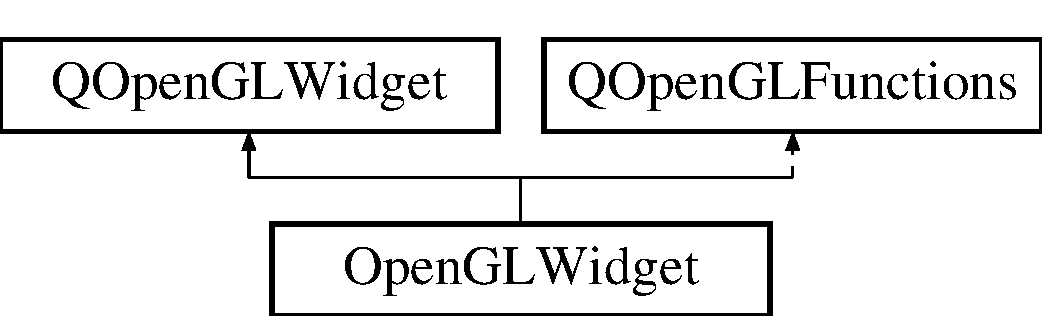
\includegraphics[height=2.000000cm]{class_open_g_l_widget}
\end{center}
\end{figure}
\subsection*{Public Member Functions}
\begin{DoxyCompactItemize}
\item 
\textbf{ Open\+G\+L\+Widget} (Q\+Widget $\ast$parent=nullptr)
\item 
\textbf{ $\sim$\+Open\+G\+L\+Widget} ()
\item 
void \textbf{ update\+Rotation} (const Q\+Vector$<$ double $>$ n\+Rotation)
\begin{DoxyCompactList}\small\item\em A method used to update the angular position of rendered object. \end{DoxyCompactList}\item 
void \textbf{ update\+Distance} (const Q\+Vector$<$ double $>$ n\+Distance)
\begin{DoxyCompactList}\small\item\em A method for updating the distance of a rendered object from the center of the coordinate system. \end{DoxyCompactList}\end{DoxyCompactItemize}
\subsection*{Protected Member Functions}
\begin{DoxyCompactItemize}
\item 
void \textbf{ initialize\+GL} () override
\begin{DoxyCompactList}\small\item\em Prepares shaders, model and it\textquotesingle{}s textures for rendering. \end{DoxyCompactList}\item 
void \textbf{ resize\+GL} (int width, int height) override
\begin{DoxyCompactList}\small\item\em Resizes widget. \end{DoxyCompactList}\item 
void \textbf{ paint\+GL} () override
\begin{DoxyCompactList}\small\item\em Draws scene. \end{DoxyCompactList}\end{DoxyCompactItemize}
\subsection*{Private Member Functions}
\begin{DoxyCompactItemize}
\item 
void \textbf{ create\+Object} ()
\begin{DoxyCompactList}\small\item\em Sends the coordinates of the vertices and UV\textquotesingle{}s of the object to the buffer. \end{DoxyCompactList}\end{DoxyCompactItemize}
\subsection*{Private Attributes}
\begin{DoxyCompactItemize}
\item 
Q\+Color \textbf{ bg\+Color}
\item 
Q\+Open\+G\+L\+Shader\+Program $\ast$ \textbf{ program}
\item 
Q\+Open\+G\+L\+Buffer \textbf{ vbo}
\item 
Q\+Vector$<$ double $>$ \textbf{ rotation}
\item 
Q\+Vector$<$ double $>$ \textbf{ distance}
\item 
\textbf{ Wireframe\+Model} $\ast$ \textbf{ model}
\item 
Q\+Open\+G\+L\+Texture $\ast$ \textbf{ texture}
\end{DoxyCompactItemize}


\subsection{Detailed Description}
A class that creates the Open\+GL window for rendering the Arduino model in real time. 

\subsection{Constructor \& Destructor Documentation}
\mbox{\label{class_open_g_l_widget_a110146940a976f19017d2747c93e0390}} 
\index{Open\+G\+L\+Widget@{Open\+G\+L\+Widget}!Open\+G\+L\+Widget@{Open\+G\+L\+Widget}}
\index{Open\+G\+L\+Widget@{Open\+G\+L\+Widget}!Open\+G\+L\+Widget@{Open\+G\+L\+Widget}}
\subsubsection{Open\+G\+L\+Widget()}
{\footnotesize\ttfamily Open\+G\+L\+Widget\+::\+Open\+G\+L\+Widget (\begin{DoxyParamCaption}\item[{Q\+Widget $\ast$}]{parent = {\ttfamily nullptr} }\end{DoxyParamCaption})\hspace{0.3cm}{\ttfamily [explicit]}}

\mbox{\label{class_open_g_l_widget_a293847f6a7e6c40344a1acfca3e9eb51}} 
\index{Open\+G\+L\+Widget@{Open\+G\+L\+Widget}!````~Open\+G\+L\+Widget@{$\sim$\+Open\+G\+L\+Widget}}
\index{````~Open\+G\+L\+Widget@{$\sim$\+Open\+G\+L\+Widget}!Open\+G\+L\+Widget@{Open\+G\+L\+Widget}}
\subsubsection{$\sim$\+Open\+G\+L\+Widget()}
{\footnotesize\ttfamily Open\+G\+L\+Widget\+::$\sim$\+Open\+G\+L\+Widget (\begin{DoxyParamCaption}{ }\end{DoxyParamCaption})}



\subsection{Member Function Documentation}
\mbox{\label{class_open_g_l_widget_ae8a75e2562bae0ea90f590f0a6ddadcc}} 
\index{Open\+G\+L\+Widget@{Open\+G\+L\+Widget}!create\+Object@{create\+Object}}
\index{create\+Object@{create\+Object}!Open\+G\+L\+Widget@{Open\+G\+L\+Widget}}
\subsubsection{create\+Object()}
{\footnotesize\ttfamily void Open\+G\+L\+Widget\+::create\+Object (\begin{DoxyParamCaption}{ }\end{DoxyParamCaption})\hspace{0.3cm}{\ttfamily [private]}}



Sends the coordinates of the vertices and UV\textquotesingle{}s of the object to the buffer. 

\mbox{\label{class_open_g_l_widget_a4baa372aec232a8d6c153cdef540dc11}} 
\index{Open\+G\+L\+Widget@{Open\+G\+L\+Widget}!initialize\+GL@{initialize\+GL}}
\index{initialize\+GL@{initialize\+GL}!Open\+G\+L\+Widget@{Open\+G\+L\+Widget}}
\subsubsection{initialize\+G\+L()}
{\footnotesize\ttfamily void Open\+G\+L\+Widget\+::initialize\+GL (\begin{DoxyParamCaption}{ }\end{DoxyParamCaption})\hspace{0.3cm}{\ttfamily [override]}, {\ttfamily [protected]}}



Prepares shaders, model and it\textquotesingle{}s textures for rendering. 

\mbox{\label{class_open_g_l_widget_a86df33a6b58b77588ffb1c110fcf2932}} 
\index{Open\+G\+L\+Widget@{Open\+G\+L\+Widget}!paint\+GL@{paint\+GL}}
\index{paint\+GL@{paint\+GL}!Open\+G\+L\+Widget@{Open\+G\+L\+Widget}}
\subsubsection{paint\+G\+L()}
{\footnotesize\ttfamily void Open\+G\+L\+Widget\+::paint\+GL (\begin{DoxyParamCaption}{ }\end{DoxyParamCaption})\hspace{0.3cm}{\ttfamily [override]}, {\ttfamily [protected]}}



Draws scene. 

\mbox{\label{class_open_g_l_widget_a1bdb72bca1dda9243983c71c8a3e0157}} 
\index{Open\+G\+L\+Widget@{Open\+G\+L\+Widget}!resize\+GL@{resize\+GL}}
\index{resize\+GL@{resize\+GL}!Open\+G\+L\+Widget@{Open\+G\+L\+Widget}}
\subsubsection{resize\+G\+L()}
{\footnotesize\ttfamily void Open\+G\+L\+Widget\+::resize\+GL (\begin{DoxyParamCaption}\item[{int}]{width,  }\item[{int}]{height }\end{DoxyParamCaption})\hspace{0.3cm}{\ttfamily [override]}, {\ttfamily [protected]}}



Resizes widget. 


\begin{DoxyParams}{Parameters}
{\em width} & \\
\hline
{\em height} & \\
\hline
\end{DoxyParams}
\mbox{\label{class_open_g_l_widget_a2170acd0e1f140dbf1771af9bf063c34}} 
\index{Open\+G\+L\+Widget@{Open\+G\+L\+Widget}!update\+Distance@{update\+Distance}}
\index{update\+Distance@{update\+Distance}!Open\+G\+L\+Widget@{Open\+G\+L\+Widget}}
\subsubsection{update\+Distance()}
{\footnotesize\ttfamily void Open\+G\+L\+Widget\+::update\+Distance (\begin{DoxyParamCaption}\item[{const Q\+Vector$<$ double $>$}]{n\+Distance }\end{DoxyParamCaption})}



A method for updating the distance of a rendered object from the center of the coordinate system. 


\begin{DoxyParams}{Parameters}
{\em n\+Distance} & -\/ x, y, z distance values \\
\hline
\end{DoxyParams}
\mbox{\label{class_open_g_l_widget_a7082dfc8237267697116a5fc03bd9a1e}} 
\index{Open\+G\+L\+Widget@{Open\+G\+L\+Widget}!update\+Rotation@{update\+Rotation}}
\index{update\+Rotation@{update\+Rotation}!Open\+G\+L\+Widget@{Open\+G\+L\+Widget}}
\subsubsection{update\+Rotation()}
{\footnotesize\ttfamily void Open\+G\+L\+Widget\+::update\+Rotation (\begin{DoxyParamCaption}\item[{const Q\+Vector$<$ double $>$}]{n\+Rotation }\end{DoxyParamCaption})}



A method used to update the angular position of rendered object. 


\begin{DoxyParams}{Parameters}
{\em n\+Rotation} & -\/ x, y, z angular position values \\
\hline
\end{DoxyParams}


\subsection{Member Data Documentation}
\mbox{\label{class_open_g_l_widget_a281ac75f22a1b4ca526be0768447fa8c}} 
\index{Open\+G\+L\+Widget@{Open\+G\+L\+Widget}!bg\+Color@{bg\+Color}}
\index{bg\+Color@{bg\+Color}!Open\+G\+L\+Widget@{Open\+G\+L\+Widget}}
\subsubsection{bg\+Color}
{\footnotesize\ttfamily Q\+Color Open\+G\+L\+Widget\+::bg\+Color\hspace{0.3cm}{\ttfamily [private]}}

\mbox{\label{class_open_g_l_widget_a6afe31b5d089a60d2f5e3e7178a7730a}} 
\index{Open\+G\+L\+Widget@{Open\+G\+L\+Widget}!distance@{distance}}
\index{distance@{distance}!Open\+G\+L\+Widget@{Open\+G\+L\+Widget}}
\subsubsection{distance}
{\footnotesize\ttfamily Q\+Vector$<$double$>$ Open\+G\+L\+Widget\+::distance\hspace{0.3cm}{\ttfamily [private]}}

\mbox{\label{class_open_g_l_widget_aa6e18f70c42656b3d8aa60f69eb761c2}} 
\index{Open\+G\+L\+Widget@{Open\+G\+L\+Widget}!model@{model}}
\index{model@{model}!Open\+G\+L\+Widget@{Open\+G\+L\+Widget}}
\subsubsection{model}
{\footnotesize\ttfamily \textbf{ Wireframe\+Model}$\ast$ Open\+G\+L\+Widget\+::model\hspace{0.3cm}{\ttfamily [private]}}

\mbox{\label{class_open_g_l_widget_a79e5c10681b015f7fb1e7ce1b047fa8b}} 
\index{Open\+G\+L\+Widget@{Open\+G\+L\+Widget}!program@{program}}
\index{program@{program}!Open\+G\+L\+Widget@{Open\+G\+L\+Widget}}
\subsubsection{program}
{\footnotesize\ttfamily Q\+Open\+G\+L\+Shader\+Program$\ast$ Open\+G\+L\+Widget\+::program\hspace{0.3cm}{\ttfamily [private]}}

\mbox{\label{class_open_g_l_widget_a3c1459d5d1e0eebd6a0eaf2e075caa1d}} 
\index{Open\+G\+L\+Widget@{Open\+G\+L\+Widget}!rotation@{rotation}}
\index{rotation@{rotation}!Open\+G\+L\+Widget@{Open\+G\+L\+Widget}}
\subsubsection{rotation}
{\footnotesize\ttfamily Q\+Vector$<$double$>$ Open\+G\+L\+Widget\+::rotation\hspace{0.3cm}{\ttfamily [private]}}

\mbox{\label{class_open_g_l_widget_afb76f6d9354bb49993c10e6fb6da7349}} 
\index{Open\+G\+L\+Widget@{Open\+G\+L\+Widget}!texture@{texture}}
\index{texture@{texture}!Open\+G\+L\+Widget@{Open\+G\+L\+Widget}}
\subsubsection{texture}
{\footnotesize\ttfamily Q\+Open\+G\+L\+Texture$\ast$ Open\+G\+L\+Widget\+::texture\hspace{0.3cm}{\ttfamily [private]}}

\mbox{\label{class_open_g_l_widget_a4b64b78f67c6da7e90cae7a4b34b5dce}} 
\index{Open\+G\+L\+Widget@{Open\+G\+L\+Widget}!vbo@{vbo}}
\index{vbo@{vbo}!Open\+G\+L\+Widget@{Open\+G\+L\+Widget}}
\subsubsection{vbo}
{\footnotesize\ttfamily Q\+Open\+G\+L\+Buffer Open\+G\+L\+Widget\+::vbo\hspace{0.3cm}{\ttfamily [private]}}



The documentation for this class was generated from the following files\+:\begin{DoxyCompactItemize}
\item 
h/\textbf{ openglwidget.\+h}\item 
cpp/\textbf{ openglwidget.\+cpp}\end{DoxyCompactItemize}

\section{Serial\+Port\+Reader Class Reference}
\label{class_serial_port_reader}\index{Serial\+Port\+Reader@{Serial\+Port\+Reader}}


A class wraps everything about receiving data from the microcontroller.  




{\ttfamily \#include $<$serialportreader.\+h$>$}

\subsection*{Public Member Functions}
\begin{DoxyCompactItemize}
\item 
\textbf{ Serial\+Port\+Reader} (\textbf{ Measurement\+Handler} $\ast$n\+Handler)
\begin{DoxyCompactList}\small\item\em Parametric constructor. \end{DoxyCompactList}\item 
\textbf{ $\sim$\+Serial\+Port\+Reader} ()
\item 
void \textbf{ read\+Line} ()
\begin{DoxyCompactList}\small\item\em A method to read one line of data from the device. \end{DoxyCompactList}\item 
Q\+Vector$<$ Q\+Serial\+Port\+Info $>$ \textbf{ get\+Info} () const
\begin{DoxyCompactList}\small\item\em A method used to obtain information about devices connected to a computer. \end{DoxyCompactList}\item 
bool \textbf{ connect} (quint32 index)
\begin{DoxyCompactList}\small\item\em A method to connect to the device via serial port. \end{DoxyCompactList}\item 
bool \textbf{ disconnect} ()
\begin{DoxyCompactList}\small\item\em A method to disconnect device from serial port. \end{DoxyCompactList}\item 
quint32 \textbf{ get\+Error\+Code} () const
\begin{DoxyCompactList}\small\item\em A method to obtain the error code. \end{DoxyCompactList}\item 
void \textbf{ reset\+Error\+Code} ()
\begin{DoxyCompactList}\small\item\em A method to remove error signatures. \end{DoxyCompactList}\end{DoxyCompactItemize}
\subsection*{Private Member Functions}
\begin{DoxyCompactItemize}
\item 
bool \textbf{ good\+Choice} ()
\begin{DoxyCompactList}\small\item\em Checks if received data from connected device is valid. \end{DoxyCompactList}\end{DoxyCompactItemize}
\subsection*{Private Attributes}
\begin{DoxyCompactItemize}
\item 
\textbf{ Measurement\+Handler} $\ast$ \textbf{ m\+Handler}
\item 
Q\+Serial\+Port $\ast$ \textbf{ m\+\_\+serial\+Port}
\item 
Q\+Vector$<$ Q\+Serial\+Port\+Info $>$ \textbf{ m\+\_\+info}
\item 
bool \textbf{ is\+Open} = false
\item 
quint32 \textbf{ error\+Code} = 0
\item 
Q\+Vector$<$ double $>$ \textbf{ time}
\item 
Q\+Vector$<$ double $>$ \textbf{ accelerationX}
\item 
Q\+Vector$<$ double $>$ \textbf{ accelerationY}
\item 
Q\+Vector$<$ double $>$ \textbf{ accelerationZ}
\item 
Q\+Vector$<$ double $>$ \textbf{ angular\+VelocityX}
\item 
Q\+Vector$<$ double $>$ \textbf{ angular\+VelocityY}
\item 
Q\+Vector$<$ double $>$ \textbf{ angular\+VelocityZ}
\end{DoxyCompactItemize}


\subsection{Detailed Description}
A class wraps everything about receiving data from the microcontroller. 

\subsection{Constructor \& Destructor Documentation}
\mbox{\label{class_serial_port_reader_aef65d0e76f65204aaa57ecfc144c827d}} 
\index{Serial\+Port\+Reader@{Serial\+Port\+Reader}!Serial\+Port\+Reader@{Serial\+Port\+Reader}}
\index{Serial\+Port\+Reader@{Serial\+Port\+Reader}!Serial\+Port\+Reader@{Serial\+Port\+Reader}}
\subsubsection{Serial\+Port\+Reader()}
{\footnotesize\ttfamily Serial\+Port\+Reader\+::\+Serial\+Port\+Reader (\begin{DoxyParamCaption}\item[{\textbf{ Measurement\+Handler} $\ast$}]{n\+Handler }\end{DoxyParamCaption})}



Parametric constructor. 


\begin{DoxyParams}{Parameters}
{\em n\+Handler} & -\/ a pointer to the object where the data of the loaded object is to be saved \\
\hline
\end{DoxyParams}
\mbox{\label{class_serial_port_reader_a7f01c445adf0d64d8acd67cd4fcd3b21}} 
\index{Serial\+Port\+Reader@{Serial\+Port\+Reader}!````~Serial\+Port\+Reader@{$\sim$\+Serial\+Port\+Reader}}
\index{````~Serial\+Port\+Reader@{$\sim$\+Serial\+Port\+Reader}!Serial\+Port\+Reader@{Serial\+Port\+Reader}}
\subsubsection{$\sim$\+Serial\+Port\+Reader()}
{\footnotesize\ttfamily Serial\+Port\+Reader\+::$\sim$\+Serial\+Port\+Reader (\begin{DoxyParamCaption}{ }\end{DoxyParamCaption})}



\subsection{Member Function Documentation}
\mbox{\label{class_serial_port_reader_ad00028795b4f33ffb0a97cd76726c4fd}} 
\index{Serial\+Port\+Reader@{Serial\+Port\+Reader}!connect@{connect}}
\index{connect@{connect}!Serial\+Port\+Reader@{Serial\+Port\+Reader}}
\subsubsection{connect()}
{\footnotesize\ttfamily bool Serial\+Port\+Reader\+::connect (\begin{DoxyParamCaption}\item[{quint32}]{index }\end{DoxyParamCaption})}



A method to connect to the device via serial port. 


\begin{DoxyParams}{Parameters}
{\em index} & -\/ device\textquotesingle{}s index \\
\hline
\end{DoxyParams}
\begin{DoxyReturn}{Returns}
true if device is succesfully connected 
\end{DoxyReturn}
\mbox{\label{class_serial_port_reader_a40d30745fd700e05d534b38c4ba4939b}} 
\index{Serial\+Port\+Reader@{Serial\+Port\+Reader}!disconnect@{disconnect}}
\index{disconnect@{disconnect}!Serial\+Port\+Reader@{Serial\+Port\+Reader}}
\subsubsection{disconnect()}
{\footnotesize\ttfamily bool Serial\+Port\+Reader\+::disconnect (\begin{DoxyParamCaption}{ }\end{DoxyParamCaption})}



A method to disconnect device from serial port. 

\begin{DoxyReturn}{Returns}
true if device is succesfully disconnected 
\end{DoxyReturn}
\mbox{\label{class_serial_port_reader_a33a6f505ebf902bf3a3f64970c6a7cec}} 
\index{Serial\+Port\+Reader@{Serial\+Port\+Reader}!get\+Error\+Code@{get\+Error\+Code}}
\index{get\+Error\+Code@{get\+Error\+Code}!Serial\+Port\+Reader@{Serial\+Port\+Reader}}
\subsubsection{get\+Error\+Code()}
{\footnotesize\ttfamily quint32 Serial\+Port\+Reader\+::get\+Error\+Code (\begin{DoxyParamCaption}{ }\end{DoxyParamCaption}) const}



A method to obtain the error code. 

\begin{DoxyReturn}{Returns}
error\textquotesingle{}s code index 
\end{DoxyReturn}
\mbox{\label{class_serial_port_reader_a5a919fb6b06f5505de1aababcde045f6}} 
\index{Serial\+Port\+Reader@{Serial\+Port\+Reader}!get\+Info@{get\+Info}}
\index{get\+Info@{get\+Info}!Serial\+Port\+Reader@{Serial\+Port\+Reader}}
\subsubsection{get\+Info()}
{\footnotesize\ttfamily Q\+Vector$<$ Q\+Serial\+Port\+Info $>$ Serial\+Port\+Reader\+::get\+Info (\begin{DoxyParamCaption}{ }\end{DoxyParamCaption}) const}



A method used to obtain information about devices connected to a computer. 

\begin{DoxyReturn}{Returns}
the device names 
\end{DoxyReturn}
\mbox{\label{class_serial_port_reader_aba5b7292f941e824467f5b1134f7f15f}} 
\index{Serial\+Port\+Reader@{Serial\+Port\+Reader}!good\+Choice@{good\+Choice}}
\index{good\+Choice@{good\+Choice}!Serial\+Port\+Reader@{Serial\+Port\+Reader}}
\subsubsection{good\+Choice()}
{\footnotesize\ttfamily bool Serial\+Port\+Reader\+::good\+Choice (\begin{DoxyParamCaption}{ }\end{DoxyParamCaption})\hspace{0.3cm}{\ttfamily [private]}}



Checks if received data from connected device is valid. 

\begin{DoxyReturn}{Returns}
true if received data is valid 
\end{DoxyReturn}
\mbox{\label{class_serial_port_reader_afb9bdbade338b204f487f2c0d4535911}} 
\index{Serial\+Port\+Reader@{Serial\+Port\+Reader}!read\+Line@{read\+Line}}
\index{read\+Line@{read\+Line}!Serial\+Port\+Reader@{Serial\+Port\+Reader}}
\subsubsection{read\+Line()}
{\footnotesize\ttfamily void Serial\+Port\+Reader\+::read\+Line (\begin{DoxyParamCaption}{ }\end{DoxyParamCaption})}



A method to read one line of data from the device. 

\mbox{\label{class_serial_port_reader_a03d89e1219ecadd67bad6a56ac6dfee2}} 
\index{Serial\+Port\+Reader@{Serial\+Port\+Reader}!reset\+Error\+Code@{reset\+Error\+Code}}
\index{reset\+Error\+Code@{reset\+Error\+Code}!Serial\+Port\+Reader@{Serial\+Port\+Reader}}
\subsubsection{reset\+Error\+Code()}
{\footnotesize\ttfamily void Serial\+Port\+Reader\+::reset\+Error\+Code (\begin{DoxyParamCaption}{ }\end{DoxyParamCaption})}



A method to remove error signatures. 



\subsection{Member Data Documentation}
\mbox{\label{class_serial_port_reader_a2224bf8c59a93b8a5ef77eace260c34c}} 
\index{Serial\+Port\+Reader@{Serial\+Port\+Reader}!accelerationX@{accelerationX}}
\index{accelerationX@{accelerationX}!Serial\+Port\+Reader@{Serial\+Port\+Reader}}
\subsubsection{accelerationX}
{\footnotesize\ttfamily Q\+Vector$<$double$>$ Serial\+Port\+Reader\+::accelerationX\hspace{0.3cm}{\ttfamily [private]}}

\mbox{\label{class_serial_port_reader_a86769450ee3907fe92dc9714f7982f26}} 
\index{Serial\+Port\+Reader@{Serial\+Port\+Reader}!accelerationY@{accelerationY}}
\index{accelerationY@{accelerationY}!Serial\+Port\+Reader@{Serial\+Port\+Reader}}
\subsubsection{accelerationY}
{\footnotesize\ttfamily Q\+Vector$<$double$>$ Serial\+Port\+Reader\+::accelerationY\hspace{0.3cm}{\ttfamily [private]}}

\mbox{\label{class_serial_port_reader_aa500a86c782f296ca529f0f4d5145366}} 
\index{Serial\+Port\+Reader@{Serial\+Port\+Reader}!accelerationZ@{accelerationZ}}
\index{accelerationZ@{accelerationZ}!Serial\+Port\+Reader@{Serial\+Port\+Reader}}
\subsubsection{accelerationZ}
{\footnotesize\ttfamily Q\+Vector$<$double$>$ Serial\+Port\+Reader\+::accelerationZ\hspace{0.3cm}{\ttfamily [private]}}

\mbox{\label{class_serial_port_reader_aeab041942a6e6178814f08315a5d73ea}} 
\index{Serial\+Port\+Reader@{Serial\+Port\+Reader}!angular\+VelocityX@{angular\+VelocityX}}
\index{angular\+VelocityX@{angular\+VelocityX}!Serial\+Port\+Reader@{Serial\+Port\+Reader}}
\subsubsection{angular\+VelocityX}
{\footnotesize\ttfamily Q\+Vector$<$double$>$ Serial\+Port\+Reader\+::angular\+VelocityX\hspace{0.3cm}{\ttfamily [private]}}

\mbox{\label{class_serial_port_reader_a5c33041effc3f958c039aceb5741c7f0}} 
\index{Serial\+Port\+Reader@{Serial\+Port\+Reader}!angular\+VelocityY@{angular\+VelocityY}}
\index{angular\+VelocityY@{angular\+VelocityY}!Serial\+Port\+Reader@{Serial\+Port\+Reader}}
\subsubsection{angular\+VelocityY}
{\footnotesize\ttfamily Q\+Vector$<$double$>$ Serial\+Port\+Reader\+::angular\+VelocityY\hspace{0.3cm}{\ttfamily [private]}}

\mbox{\label{class_serial_port_reader_a906e4e7d144d9a105fc8d4f31fcf40e9}} 
\index{Serial\+Port\+Reader@{Serial\+Port\+Reader}!angular\+VelocityZ@{angular\+VelocityZ}}
\index{angular\+VelocityZ@{angular\+VelocityZ}!Serial\+Port\+Reader@{Serial\+Port\+Reader}}
\subsubsection{angular\+VelocityZ}
{\footnotesize\ttfamily Q\+Vector$<$double$>$ Serial\+Port\+Reader\+::angular\+VelocityZ\hspace{0.3cm}{\ttfamily [private]}}

\mbox{\label{class_serial_port_reader_a40153d2e5ce2b54838b9ba25c2316340}} 
\index{Serial\+Port\+Reader@{Serial\+Port\+Reader}!error\+Code@{error\+Code}}
\index{error\+Code@{error\+Code}!Serial\+Port\+Reader@{Serial\+Port\+Reader}}
\subsubsection{error\+Code}
{\footnotesize\ttfamily quint32 Serial\+Port\+Reader\+::error\+Code = 0\hspace{0.3cm}{\ttfamily [private]}}

\mbox{\label{class_serial_port_reader_a944ec89d2b0aa1a27e873c77cfbaf355}} 
\index{Serial\+Port\+Reader@{Serial\+Port\+Reader}!is\+Open@{is\+Open}}
\index{is\+Open@{is\+Open}!Serial\+Port\+Reader@{Serial\+Port\+Reader}}
\subsubsection{is\+Open}
{\footnotesize\ttfamily bool Serial\+Port\+Reader\+::is\+Open = false\hspace{0.3cm}{\ttfamily [private]}}

\mbox{\label{class_serial_port_reader_a2c2207d575acd7adc3746e514a00e819}} 
\index{Serial\+Port\+Reader@{Serial\+Port\+Reader}!m\+\_\+info@{m\+\_\+info}}
\index{m\+\_\+info@{m\+\_\+info}!Serial\+Port\+Reader@{Serial\+Port\+Reader}}
\subsubsection{m\+\_\+info}
{\footnotesize\ttfamily Q\+Vector$<$Q\+Serial\+Port\+Info$>$ Serial\+Port\+Reader\+::m\+\_\+info\hspace{0.3cm}{\ttfamily [private]}}

\mbox{\label{class_serial_port_reader_a07a8c1715274118e7886f671f287c3ec}} 
\index{Serial\+Port\+Reader@{Serial\+Port\+Reader}!m\+\_\+serial\+Port@{m\+\_\+serial\+Port}}
\index{m\+\_\+serial\+Port@{m\+\_\+serial\+Port}!Serial\+Port\+Reader@{Serial\+Port\+Reader}}
\subsubsection{m\+\_\+serial\+Port}
{\footnotesize\ttfamily Q\+Serial\+Port$\ast$ Serial\+Port\+Reader\+::m\+\_\+serial\+Port\hspace{0.3cm}{\ttfamily [private]}}

\mbox{\label{class_serial_port_reader_a2ee8eead177a8d309115708a4ca354d0}} 
\index{Serial\+Port\+Reader@{Serial\+Port\+Reader}!m\+Handler@{m\+Handler}}
\index{m\+Handler@{m\+Handler}!Serial\+Port\+Reader@{Serial\+Port\+Reader}}
\subsubsection{m\+Handler}
{\footnotesize\ttfamily \textbf{ Measurement\+Handler}$\ast$ Serial\+Port\+Reader\+::m\+Handler\hspace{0.3cm}{\ttfamily [private]}}

\mbox{\label{class_serial_port_reader_ac023d7fa3c67e9e9d3d20e73249312c5}} 
\index{Serial\+Port\+Reader@{Serial\+Port\+Reader}!time@{time}}
\index{time@{time}!Serial\+Port\+Reader@{Serial\+Port\+Reader}}
\subsubsection{time}
{\footnotesize\ttfamily Q\+Vector$<$double$>$ Serial\+Port\+Reader\+::time\hspace{0.3cm}{\ttfamily [private]}}



The documentation for this class was generated from the following files\+:\begin{DoxyCompactItemize}
\item 
h/\textbf{ serialportreader.\+h}\item 
cpp/\textbf{ serialportreader.\+cpp}\end{DoxyCompactItemize}

\section{Wireframe\+Model Class Reference}
\label{class_wireframe_model}\index{Wireframe\+Model@{Wireframe\+Model}}


A class that loads data from a file and stores it for rendering using Open\+GL.  




{\ttfamily \#include $<$wireframemodel.\+h$>$}

\subsection*{Public Member Functions}
\begin{DoxyCompactItemize}
\item 
\textbf{ Wireframe\+Model} ()
\item 
\textbf{ $\sim$\+Wireframe\+Model} ()
\item 
bool \textbf{ Load\+Object} (const Q\+String filename)
\begin{DoxyCompactList}\small\item\em A method for parsing and saving a 3D model. \end{DoxyCompactList}\item 
Q\+Vector$<$ G\+Lfloat $>$ $\ast$ \textbf{ get\+Data} () const
\begin{DoxyCompactList}\small\item\em Getter for object\textquotesingle{}s data. \end{DoxyCompactList}\item 
quint32 \textbf{ get\+Size} () const
\begin{DoxyCompactList}\small\item\em Getter for amount of stored vertices and UV\textquotesingle{}s combined. \end{DoxyCompactList}\end{DoxyCompactItemize}
\subsection*{Private Attributes}
\begin{DoxyCompactItemize}
\item 
Q\+Vector$<$ G\+Lfloat $>$ $\ast$ \textbf{ data}
\end{DoxyCompactItemize}


\subsection{Detailed Description}
A class that loads data from a file and stores it for rendering using Open\+GL. 

\subsection{Constructor \& Destructor Documentation}
\mbox{\label{class_wireframe_model_aab69007d1aea9e74f8639d6264e6b61f}} 
\index{Wireframe\+Model@{Wireframe\+Model}!Wireframe\+Model@{Wireframe\+Model}}
\index{Wireframe\+Model@{Wireframe\+Model}!Wireframe\+Model@{Wireframe\+Model}}
\subsubsection{Wireframe\+Model()}
{\footnotesize\ttfamily Wireframe\+Model\+::\+Wireframe\+Model (\begin{DoxyParamCaption}{ }\end{DoxyParamCaption})}

\mbox{\label{class_wireframe_model_a57ec6b8bf2a697a074903d42e4db90d4}} 
\index{Wireframe\+Model@{Wireframe\+Model}!````~Wireframe\+Model@{$\sim$\+Wireframe\+Model}}
\index{````~Wireframe\+Model@{$\sim$\+Wireframe\+Model}!Wireframe\+Model@{Wireframe\+Model}}
\subsubsection{$\sim$\+Wireframe\+Model()}
{\footnotesize\ttfamily Wireframe\+Model\+::$\sim$\+Wireframe\+Model (\begin{DoxyParamCaption}{ }\end{DoxyParamCaption})}



\subsection{Member Function Documentation}
\mbox{\label{class_wireframe_model_a1d20cf72b2f6412985f5fa2fddcec3ee}} 
\index{Wireframe\+Model@{Wireframe\+Model}!get\+Data@{get\+Data}}
\index{get\+Data@{get\+Data}!Wireframe\+Model@{Wireframe\+Model}}
\subsubsection{get\+Data()}
{\footnotesize\ttfamily Q\+Vector$<$ G\+Lfloat $>$ $\ast$ Wireframe\+Model\+::get\+Data (\begin{DoxyParamCaption}{ }\end{DoxyParamCaption}) const}



Getter for object\textquotesingle{}s data. 

\begin{DoxyReturn}{Returns}
Pointer to object\textquotesingle{}s data 
\end{DoxyReturn}
\mbox{\label{class_wireframe_model_a5fc0323e4618b80e1b2b227f2470b6a0}} 
\index{Wireframe\+Model@{Wireframe\+Model}!get\+Size@{get\+Size}}
\index{get\+Size@{get\+Size}!Wireframe\+Model@{Wireframe\+Model}}
\subsubsection{get\+Size()}
{\footnotesize\ttfamily quint32 Wireframe\+Model\+::get\+Size (\begin{DoxyParamCaption}{ }\end{DoxyParamCaption}) const}



Getter for amount of stored vertices and UV\textquotesingle{}s combined. 

\begin{DoxyReturn}{Returns}
Size of data container 
\end{DoxyReturn}
\mbox{\label{class_wireframe_model_ac5f8817ea433184dda70ee25633043ae}} 
\index{Wireframe\+Model@{Wireframe\+Model}!Load\+Object@{Load\+Object}}
\index{Load\+Object@{Load\+Object}!Wireframe\+Model@{Wireframe\+Model}}
\subsubsection{Load\+Object()}
{\footnotesize\ttfamily bool Wireframe\+Model\+::\+Load\+Object (\begin{DoxyParamCaption}\item[{const Q\+String}]{filename }\end{DoxyParamCaption})}



A method for parsing and saving a 3D model. 


\begin{DoxyParams}{Parameters}
{\em filename} & -\/ path for file .obj, extension not included \\
\hline
\end{DoxyParams}
\begin{DoxyReturn}{Returns}
true if model is loaded succesfully 
\end{DoxyReturn}


\subsection{Member Data Documentation}
\mbox{\label{class_wireframe_model_a9fb28b2dedbdcfff31c9ccc592b8492a}} 
\index{Wireframe\+Model@{Wireframe\+Model}!data@{data}}
\index{data@{data}!Wireframe\+Model@{Wireframe\+Model}}
\subsubsection{data}
{\footnotesize\ttfamily Q\+Vector$<$G\+Lfloat$>$$\ast$ Wireframe\+Model\+::data\hspace{0.3cm}{\ttfamily [private]}}



The documentation for this class was generated from the following files\+:\begin{DoxyCompactItemize}
\item 
h/\textbf{ wireframemodel.\+h}\item 
cpp/\textbf{ wireframemodel.\+cpp}\end{DoxyCompactItemize}

\chapter{File Documentation}
\section{cpp/main.cpp File Reference}
\label{main_8cpp}\index{cpp/main.\+cpp@{cpp/main.\+cpp}}
{\ttfamily \#include \char`\"{}mainwindow.\+h\char`\"{}}\newline
{\ttfamily \#include $<$Q\+Application$>$}\newline
{\ttfamily \#include $<$Q\+Surface\+Format$>$}\newline
\subsection*{Functions}
\begin{DoxyCompactItemize}
\item 
int \textbf{ main} (int argc, char $\ast$argv[$\,$])
\end{DoxyCompactItemize}


\subsection{Function Documentation}
\mbox{\label{main_8cpp_a0ddf1224851353fc92bfbff6f499fa97}} 
\index{main.\+cpp@{main.\+cpp}!main@{main}}
\index{main@{main}!main.\+cpp@{main.\+cpp}}
\subsubsection{main()}
{\footnotesize\ttfamily int main (\begin{DoxyParamCaption}\item[{int}]{argc,  }\item[{char $\ast$}]{argv[$\,$] }\end{DoxyParamCaption})}


\section{cpp/mainwindow.cpp File Reference}
\label{mainwindow_8cpp}\index{cpp/mainwindow.\+cpp@{cpp/mainwindow.\+cpp}}
{\ttfamily \#include \char`\"{}mainwindow.\+h\char`\"{}}\newline
{\ttfamily \#include \char`\"{}ui\+\_\+mainwindow.\+h\char`\"{}}\newline

\section{cpp/measurementhandler.cpp File Reference}
\label{measurementhandler_8cpp}\index{cpp/measurementhandler.\+cpp@{cpp/measurementhandler.\+cpp}}
{\ttfamily \#include \char`\"{}measurementhandler.\+h\char`\"{}}\newline

\section{cpp/openglwidget.cpp File Reference}
\label{openglwidget_8cpp}\index{cpp/openglwidget.\+cpp@{cpp/openglwidget.\+cpp}}
{\ttfamily \#include \char`\"{}openglwidget.\+h\char`\"{}}\newline
\subsection*{Macros}
\begin{DoxyCompactItemize}
\item 
\#define \textbf{ V\+E\+R\+T\+E\+X\+\_\+\+C\+O\+O\+R\+D\+\_\+\+A\+T\+T\+R\+I\+B\+U\+TE}~0
\item 
\#define \textbf{ T\+E\+X\+T\+U\+R\+E\+\_\+\+C\+O\+O\+R\+D\+\_\+\+A\+T\+T\+R\+I\+B\+U\+TE}~1
\end{DoxyCompactItemize}


\subsection{Macro Definition Documentation}
\mbox{\label{openglwidget_8cpp_acff437f714a20ac71a7bf4f8fa570d2c}} 
\index{openglwidget.\+cpp@{openglwidget.\+cpp}!T\+E\+X\+T\+U\+R\+E\+\_\+\+C\+O\+O\+R\+D\+\_\+\+A\+T\+T\+R\+I\+B\+U\+TE@{T\+E\+X\+T\+U\+R\+E\+\_\+\+C\+O\+O\+R\+D\+\_\+\+A\+T\+T\+R\+I\+B\+U\+TE}}
\index{T\+E\+X\+T\+U\+R\+E\+\_\+\+C\+O\+O\+R\+D\+\_\+\+A\+T\+T\+R\+I\+B\+U\+TE@{T\+E\+X\+T\+U\+R\+E\+\_\+\+C\+O\+O\+R\+D\+\_\+\+A\+T\+T\+R\+I\+B\+U\+TE}!openglwidget.\+cpp@{openglwidget.\+cpp}}
\subsubsection{T\+E\+X\+T\+U\+R\+E\+\_\+\+C\+O\+O\+R\+D\+\_\+\+A\+T\+T\+R\+I\+B\+U\+TE}
{\footnotesize\ttfamily \#define T\+E\+X\+T\+U\+R\+E\+\_\+\+C\+O\+O\+R\+D\+\_\+\+A\+T\+T\+R\+I\+B\+U\+TE~1}

\mbox{\label{openglwidget_8cpp_a3d917d14a52acad99a52b2ade787e7e6}} 
\index{openglwidget.\+cpp@{openglwidget.\+cpp}!V\+E\+R\+T\+E\+X\+\_\+\+C\+O\+O\+R\+D\+\_\+\+A\+T\+T\+R\+I\+B\+U\+TE@{V\+E\+R\+T\+E\+X\+\_\+\+C\+O\+O\+R\+D\+\_\+\+A\+T\+T\+R\+I\+B\+U\+TE}}
\index{V\+E\+R\+T\+E\+X\+\_\+\+C\+O\+O\+R\+D\+\_\+\+A\+T\+T\+R\+I\+B\+U\+TE@{V\+E\+R\+T\+E\+X\+\_\+\+C\+O\+O\+R\+D\+\_\+\+A\+T\+T\+R\+I\+B\+U\+TE}!openglwidget.\+cpp@{openglwidget.\+cpp}}
\subsubsection{V\+E\+R\+T\+E\+X\+\_\+\+C\+O\+O\+R\+D\+\_\+\+A\+T\+T\+R\+I\+B\+U\+TE}
{\footnotesize\ttfamily \#define V\+E\+R\+T\+E\+X\+\_\+\+C\+O\+O\+R\+D\+\_\+\+A\+T\+T\+R\+I\+B\+U\+TE~0}


\hypertarget{serialportreader_8cpp}{}\section{cpp/serialportreader.cpp File Reference}
\label{serialportreader_8cpp}\index{cpp/serialportreader.\+cpp@{cpp/serialportreader.\+cpp}}
{\ttfamily \#include \char`\"{}serialportreader.\+h\char`\"{}}\newline
{\ttfamily \#include $<$Q\+Core\+Application$>$}\newline

\section{cpp/wireframemodel.cpp File Reference}
\label{wireframemodel_8cpp}\index{cpp/wireframemodel.\+cpp@{cpp/wireframemodel.\+cpp}}
{\ttfamily \#include \char`\"{}wireframemodel.\+h\char`\"{}}\newline

\section{h/mainwindow.h File Reference}
\label{mainwindow_8h}\index{h/mainwindow.\+h@{h/mainwindow.\+h}}
{\ttfamily \#include $<$Q\+Main\+Window$>$}\newline
{\ttfamily \#include $<$Q\+Debug$>$}\newline
{\ttfamily \#include $<$Q\+Timer$>$}\newline
{\ttfamily \#include $<$Q\+Color$>$}\newline
{\ttfamily \#include $<$Qt\+Math$>$}\newline
{\ttfamily \#include \char`\"{}qcustomplot.\+h\char`\"{}}\newline
{\ttfamily \#include \char`\"{}ledindicator.\+h\char`\"{}}\newline
{\ttfamily \#include \char`\"{}serialportreader.\+h\char`\"{}}\newline
{\ttfamily \#include \char`\"{}measurementhandler.\+h\char`\"{}}\newline
\subsection*{Classes}
\begin{DoxyCompactItemize}
\item 
class \textbf{ Main\+Window}
\begin{DoxyCompactList}\small\item\em A class that supports the user interface and a module that generates charts. \end{DoxyCompactList}\end{DoxyCompactItemize}
\subsection*{Namespaces}
\begin{DoxyCompactItemize}
\item 
 \textbf{ Ui}
\end{DoxyCompactItemize}

\hypertarget{measurementhandler_8h}{}\section{h/measurementhandler.h File Reference}
\label{measurementhandler_8h}\index{h/measurementhandler.\+h@{h/measurementhandler.\+h}}
{\ttfamily \#include $<$Q\+Vector$>$}\newline
{\ttfamily \#include $<$Q\+Debug$>$}\newline
{\ttfamily \#include $<$Qt\+Math$>$}\newline
\subsection*{Classes}
\begin{DoxyCompactItemize}
\item 
class \mbox{\hyperlink{class_measurement_handler}{Measurement\+Handler}}
\begin{DoxyCompactList}\small\item\em A class for storing data from sensors received from the microcontroller and handling necessary conversions. \end{DoxyCompactList}\end{DoxyCompactItemize}

\section{h/openglwidget.h File Reference}
\label{openglwidget_8h}\index{h/openglwidget.\+h@{h/openglwidget.\+h}}
{\ttfamily \#include $<$Q\+Widget$>$}\newline
{\ttfamily \#include $<$Q\+Open\+G\+L\+Functions$>$}\newline
{\ttfamily \#include $<$Q\+Open\+G\+L\+Widget$>$}\newline
{\ttfamily \#include $<$Q\+Open\+G\+L\+Buffer$>$}\newline
{\ttfamily \#include $<$Q\+Open\+G\+L\+Shader\+Program$>$}\newline
{\ttfamily \#include $<$Q\+Matrix4x4$>$}\newline
{\ttfamily \#include $<$Q\+Quaternion$>$}\newline
{\ttfamily \#include $<$Q\+Vector$>$}\newline
{\ttfamily \#include $<$Q\+Open\+G\+L\+Texture$>$}\newline
{\ttfamily \#include \char`\"{}wireframemodel.\+h\char`\"{}}\newline
\subsection*{Classes}
\begin{DoxyCompactItemize}
\item 
class \textbf{ Open\+G\+L\+Widget}
\begin{DoxyCompactList}\small\item\em A class that creates the Open\+GL window for rendering the Arduino model in real time. \end{DoxyCompactList}\end{DoxyCompactItemize}

\hypertarget{serialportreader_8h}{}\section{h/serialportreader.h File Reference}
\label{serialportreader_8h}\index{h/serialportreader.\+h@{h/serialportreader.\+h}}
{\ttfamily \#include $<$Q\+Byte\+Array$>$}\newline
{\ttfamily \#include $<$Q\+Serial\+Port$>$}\newline
{\ttfamily \#include $<$Q\+Serial\+Port\+Info$>$}\newline
{\ttfamily \#include $<$Q\+Debug$>$}\newline
{\ttfamily \#include $<$Q\+Vector3D$>$}\newline
{\ttfamily \#include $<$Q\+String$>$}\newline
{\ttfamily \#include $<$Q\+String\+List$>$}\newline
{\ttfamily \#include \char`\"{}measurementhandler.\+h\char`\"{}}\newline
{\ttfamily \#include $<$Q\+Application$>$}\newline
{\ttfamily \#include $<$Q\+Thread$>$}\newline
\subsection*{Classes}
\begin{DoxyCompactItemize}
\item 
class \mbox{\hyperlink{class_serial_port_reader}{Serial\+Port\+Reader}}
\begin{DoxyCompactList}\small\item\em A class wraps everything about receiving data from the microcontroller. \end{DoxyCompactList}\end{DoxyCompactItemize}

\hypertarget{wireframemodel_8h}{}\section{h/wireframemodel.h File Reference}
\label{wireframemodel_8h}\index{h/wireframemodel.\+h@{h/wireframemodel.\+h}}
{\ttfamily \#include $<$Q\+String$>$}\newline
{\ttfamily \#include $<$Q\+Vector$>$}\newline
{\ttfamily \#include $<$Q\+Vector3D$>$}\newline
{\ttfamily \#include $<$Q\+Vector2D$>$}\newline
{\ttfamily \#include $<$Q\+File$>$}\newline
{\ttfamily \#include $<$Q\+Debug$>$}\newline
{\ttfamily \#include $<$Q\+Open\+G\+L\+Functions$>$}\newline
\subsection*{Classes}
\begin{DoxyCompactItemize}
\item 
class \mbox{\hyperlink{class_wireframe_model}{Wireframe\+Model}}
\begin{DoxyCompactList}\small\item\em A class that loads data from a file and stores it for rendering using Open\+GL. \end{DoxyCompactList}\end{DoxyCompactItemize}

%--- End generated contents ---

% Index
\backmatter
\newpage
\phantomsection
\clearemptydoublepage
\addcontentsline{toc}{chapter}{Index}
\printindex

\end{document}
